\documentclass[preprint,12pt]{elsarticle}

\usepackage{amssymb}
\usepackage{amsmath}
\usepackage{multirow}
\usepackage{algorithm}
\usepackage{adjustbox}
\usepackage{algpseudocode}

\journal{Neurocomputing}

\begin{document}

\begin{frontmatter}

\title{AdaGrow: An Task-Adaptive Model Growing Framework for Efficient Convolutional Neural Networks}

\author{Guanchen Li, Jie He, Yue Qi} 

\affiliation{organization={School of Computer and Communication Engineering, University of Science and Technology Beijing},
            addressline={Xueyuan Road 30, Haidian}, 
            city={Beijing},
            postcode={100083}, 
            % state={},
            country={China}}

%% Abstract
\begin{abstract}
Neural network design typically follows a paradigm of preset model sizes and pre-training, requiring users to customize these models to meet dynamic task requirements and inference efficiency. We propose the AdaGrow framework to address this issue. It progressively expands the model size during training to achieve task adaptation, balancing performance and efficiency. AdaGrow focuses on adding richer feature extraction structures to critical parts of the model and explores key factors affecting model growing, including depth and width growing strategies, growing frequency, termination conditions, module initialization, and optimizer alignment. Among its features, AdaGrow employs structural re-parameterization technology to simulate width growing, avoiding efficiency losses from actual width expansion. Additionally, we introduce an innovative quantization method to address high quantization losses caused by less over-parameterization and abnormal weight distribution resulting from re-parameterization. This method effectively reduces performance loss through error compensation and weight reordering, facilitating efficient deployment of grown networks. Experimental results demonstrate that AdaGrow achieves an average improvement of 10.75\% in accuracy and 40.4\% in inference speed across eight vision recognition tasks compared to the best fixed-size models. Additionally, AdaGrow surpasses model pruning and other model growing methods by 2.7\% in accuracy and 45.9\% in inference speed. Under identical quantization configurations, our optimized quantization method improves accuracy by 0.7\% on average over vanilla ones.
\end{abstract}


\begin{highlights}
\item We achieve task adaptability and performance-efficiency trade-off with a novel model growing framework AdaGrow.
\item We enhance the efficiency and performance of growing convolutional neural networks through structural re-parameterization: simulating width growing without increasing actual width.
\item We address quantization challenges in grown models, including issues from less over-parameterization and abnormal weight distribution from re-parameterization, with optimized quantization methods based on error compensation and weight reordering.
\item Experimental results show that the AdaGrow framework improves accuracy by 10.75\% and inference speed by 40.4\% on average across eight vision recognition tasks compared to fixed-size models, surpassing pruning and other growing methods. Our optimized quantization method improves accuracy by an average of 0.7\% compared to vanilla ones.
\end{highlights}

%% Keywords
\begin{keyword}
Task adaptation \sep Model growing \sep Structural re-parameterization \sep Model compression

\end{keyword}

\end{frontmatter}

\section{Introduction}
\label{introduction}
As deep learning technology advances, model design is evolving towards larger scales and more complex structures. Notwithstanding this, most models currently, whether Convolutional Neural Networks (CNNs) \cite{cnn} or Transformer architectures \cite{transformer}, are designed with fixed sizes \cite{fixscale}.

However, in fields requiring high recognition accuracy and speed, such as autonomous driving \cite{autodrive}, deploying fixed-size neural networks presents significant challenges. These models, including various versions like \textit{base}, \textit{large}, or \textit{xlarge}, often fail to adapt adequately to the specific needs of different tasks, leading to unnecessary compromises in performance or computational efficiency, for example, an user-customized task might require a ResNet33, which does not match the available ResNet18 or ResNet50 models. Additionally, users may struggle to determine that ResNet33 is the optimal size for their specific task. Furthermore, training a fixed-size network from scratch, especially a large one, may present more local minima and saddle points in the loss surface, complicating parameter initialization and optimization \cite{hardtrain}. To address these challenges, methods like lightweight neural network design \cite{lightweight}, pruning \cite{pruning}, and quantization \cite{quantization} have been explored. These model compression strategies, which often follow a \textit{pre-training}, \textit{compression}, \textit{fine-tuning} optimization process, aim to balance accuracy and speed. However, they often lead to performance compromises and may depend on complex search or fine-tuning processes \cite{finetuning}.

Unlike the fixed-size design of neural networks, the brain's capacity and the number of neuron connections increase as it matures \cite{brain}, providing inspiration for model growing. Model growing, a subfield of neural architecture search \cite{nas}, gradually expands model size during training processes. This approach has the potential to find the optimal balance between performance and efficiency for specific tasks. Current research on model growing is in its very early stages, focusing primarily on growing strategy design. Emerging strategies include random depth growing \cite{autogrow}, maintaining computational equivalence before and after width growing \cite{splitgrow}, and using the momentum of existing network modules to initialize new ones \cite{mogrow}. While these strategies have shown promising experimental results, significant gaps remain in comprehensiveness, depth-width growing matching, and lower-scale network search.

Recognizing the powerful advantage of model growing in ensuring task adaptability while reducing manual architecture adjustments and resource consumption, this study aims to explore more efficient task-adaptive convolutional neural networks. Thus, this study proposes a task-adaptive model growing method named AdaGrow, which progressively enlarges the neural network model during training to achieve an optimal balance between performance and efficiency for specific tasks. Specifically, this research aims to add functionally diverse feature extraction structures to critical positions in the model, addressing several key challenges: determining the frequency of model growing, identifying which parts of the model should be expanded, selecting new network modules for growing, allocating width and depth growing, initializing new network modules, and optimizing the expanded model. AdaGrow introduces a novel training framework that allows neural networks to progressively grow to a size suitable for specific tasks during training. Compared to directly training fixed-size models, this approach significantly improves training speed, reduces training complexity (including simplifications in regularization, learning rate, and optimizer design), and enhances model adaptability to specific tasks. This study further investigates the balance between performance and efficiency for convolutional neural networks through structural re-parameterization. By adding re-parameterizable branches to layers, we achieves simulated network width growing. This method avoids the efficiency reduction typically associated with direct width increases while ensuring effective performance improvement. Conventional model quantization methods rely on model over-parameterization to explore compression space, which leads to challenges in effectively quantizing grown models where over-parameterization is less pronounced. Structural reparameterization introduces anomalous weight distribution phenomena to the grown model, further increasing the challenge of model quantification. This research provide a novel quantization method based on loss compensation and weight reordering, thereby enhancing the performance of the quantized model and improving the efficiency of grown models in practical deployment. 

This comprehensive approach ensures that the grown models are not only adaptable to specific tasks but also maintain high performance and efficiency: Experimental results demonstrate that the AdaGrow framework enhances accuracy by 10.75\% and inference speed by 40.4\% on average across eight vision recognition tasks compared to fixed-size models, outperforming pruning and other model growing methods. Additionally, our optimized quantization method, which incorporates loss compensation and weight reordering, improves accuracy by an average of 0.7\% compared to standard quantization methods.

\section{Related Works}
\label{related_works}

\textbf{Convolutional Neural Networks} \cite{cnn} have revolutionized computer vision tasks due to their ability to automatically learn hierarchical features from data. VGG networks introduced a simple yet effective architecture with deep stacks of convolutional layers, achieving remarkable accuracy on image recognition benchmarks \cite{vgg}. ResNet further advanced this field by incorporating residual learning, which mitigates the vanishing gradient problem and allows for training much deeper networks \cite{resnet}. The introduction of bottleneck layers in ResNet variants improved computational efficiency by reducing the number of parameters while maintaining high performance. MobileNet series, including v1 \cite{mobilenet1}, v2 \cite{mobilenet2}, and v3 \cite{mobilenet3}, focused on optimizing CNNs for mobile and embedded devices by employing depthwise separable convolutions and linear bottlenecks, significantly reducing model size and inference time without compromising accuracy. These innovations underscore the continuous evolution of CNN architectures, driving advancements in both model performance and efficiency.

\textbf{Model optimization} techniques such as pruning \cite{pruning}, quantization \cite{quantization}, structural re-parameterization \cite{acnet}, neural architecture search \cite{nas}, and model growing \cite{autogrow} have been developed to pursue higher efficiency. These methods aim to reduce computational complexity and resource consumption while maintaining or even enhancing model performance, addressing the increasing demand for efficient and scalable solutions in diverse applications.

\textbf{Pruning} \cite{pruning} is a model compression and inference acceleration technique that reduces the number of parameters in a neural network by trimming its structure, thereby decreasing computational load and runtime resource consumption with minimal performance loss. Pruning can be categorized into structured, unstructured, and semi-structured pruning. Structured pruning targets entire network structures like convolutional channels or fully connected layers, with notable methods including Liu's batch normalization-based approach \cite{bnpruning} and He et al.'s channel pruning using ridge regression \cite{channelpruning}. Unstructured pruning, which sparsifies the weight matrix elements, is exemplified by Han's Deep Compression technique \cite{deepc} and the recent SparseGPT framework \cite{sparsegpt}. Semi-structured pruning, or N:M sparsity, strikes a balance between the two by enforcing a fixed sparsity pattern, as demonstrated by the R-TOSS framework for real-time object detection \cite{RTOSS}. These pruning strategies collectively aim to enhance efficiency while maintaining model performance across various applications.

\textbf{Quantization} \cite{quantization} is a technique that reduces the storage and computational complexity of deep learning models by decreasing the bit-width of model weights and activations. It is particularly important for deploying models on embedded systems and mobile devices with limited computational resources and storage. Quantization can be divided into symmetric and asymmetric types. Symmetric quantization uses a single scale factor, while asymmetric quantization incorporates both a scale factor and a zero-point, allowing for more flexible and accurate mapping. Key methods include ZeroQ, which synthesizes data to achieve high-precision quantization without original training data \cite{zeroq}, and AdaRound, which learns optimal rounding thresholds for each weight to reduce quantization error \cite{adaround}. Techniques like LSQ+ improve performance in low-bit quantization by optimizing quantization intervals and functions \cite{lsq}. For Vision Transformers, Q-vit effectively reduces computational complexity while maintaining visual processing performance \cite{qvit}. These advancements demonstrate the versatility and effectiveness of quantization in enhancing model efficiency and deployment feasibility.

\textbf{Structural re-parameterization} \cite{acnet} transforms a complex training architecture into a simpler inference architecture while maintaining linear equivalence, enhancing feature extraction during training and ensuring efficient inference. This technique often merges convolution and batch normalization layers, simplifying the model without sacrificing performance. Notable methods include ACNet, which uses parallel convolution layers of varying sizes to enhance feature extraction \cite{acnet}, and DBB, which integrates diverse branches, including convolutions and pooling layers, for robust feature extraction \cite{dbb}. RepVGG combines ResNet-like training with VGG-like inference by re-parameterizing multiple branches into a single convolutional layer \cite{repvgg}. These approaches demonstrate the effectiveness of structural re-parameterization in improving both model performance and inference efficiency.

\textbf{Neural Architecture Search (NAS)} \cite{nas} is an automated approach aimed at discovering more efficient and high-performing model architectures, surpassing human-designed models. NAS involves defining the search space, employing search strategies such as gradient-based, evolutionary/genetic algorithms, and reinforcement learning, and utilizing performance evaluation strategies. Although NAS is computationally intensive, it significantly reduces the time and expertise required for network design. Key advancements include EfficientNet, which uses a compound model scaling method to balance width, depth, and resolution for improved efficiency and accuracy \cite{efficientnet}; DARTS, a gradient-based method that optimizes architectures in a continuous search space, accelerating the search process and reducing costs \cite{darts}; and MnasNet, which introduces a platform-aware objective function to balance accuracy and efficiency for mobile devices \cite{mnasnet}. Once for All trains a supernet with diverse design choices, allowing subnetwork optimization for different deployment scenarios without retraining \cite{once}. AutoML-Zero employs evolutionary algorithms to discover machine learning algorithms from basic operations, exploring novel algorithm structures \cite{automlz}. ENAS reduces computational cost through parameter sharing, enabling efficient architecture search on standard hardware \cite{enas}. FBNet uses a differentiable NAS framework to design convolutional networks with hardware constraints, optimizing for specific configurations to ensure high performance and efficiency \cite{fbnet}. These developments highlight NAS's potential in automating and enhancing neural network design.

\textbf{Model growing} \cite{autogrow}, a key focus of this study within the Neural Architecture Search (NAS) field, aims to reduce the computational costs associated with training neural networks. Unlike traditional NAS, which requires extensive computational resources, model growing incrementally expands the network during training. This approach is in its early stages, with notable methods including Duke University's random depth-based model growing, which initializes and expands modules randomly or sequentially to achieve better performance and faster training than training a fixed-size network from scratch \cite{autogrow}. MoGrow introduces momentum growing and adaptive training load strategies to accelerate training for Vision Transformer (ViT) models without performance loss, significantly reducing search costs \cite{mogrow}. SplitGrow addresses training imbalances caused by network growing through dynamic parameter scaling and learning rate adaptation, achieving accuracy comparable to large fixed models with less computational budget \cite{splitgrow}. MixtureGrowth reassembles pre-trained small model modules for network expansion, retaining strong initialization while allowing new layers to learn flexibly \cite{mixturegrowth}. GROWN employs sparse growing, dynamically expanding the model only when necessary, outperforming traditional methods in both accuracy and model size across multiple tasks \cite{grown}. The DNNDeepeningPruning algorithm generates compact neural network architectures for medical imaging diagnostics by deepening and pruning residual blocks, improving efficiency and accuracy \cite{DNNDeepeningPruning}. These advancements demonstrate the potential of model growing in creating efficient, scalable neural networks.


Model growing addresses the challenges of resource constraints and low computational efficiency faced by advanced neural networks. Unlike traditional model compression methods, model growing incrementally expands the network, allowing for more efficient and scalable architectures. Our proposed AdaGrow method improves upon existing techniques by providing a more targeted and strategic approach to network expansion, considering both depth and width, optimizing structural choices, growing locations, and post-expansion optimizations. AdaGrow ensures efficient resource usage and enhances performance, offering a streamlined solution to achieve high-performance, compact neural networks tailored to specific tasks.


\section{AdaGrow: Task-Adaptive Model Growing Framework}
\label{method}

\subsection{Framework}

In the human brain's developmental process, brain capacity and neuron connections continuously increase with age, demonstrating a natural growing model of intelligent organisms \cite{brain}. In contrast, modern artificial neural networks are typically designed with fixed sizes before training, which limits their learning ability and adaptability. Static neural network designs face several challenges: training a fixed-size network from scratch, especially a large one, can lead to numerous local minima and saddle points in the loss landscape, complicating parameter initialization and optimization. Additionally, pre-trained models usually come in fixed sizes (e.g., ResNet18, ResNet50), which may not suit specific task requirements, forcing users to design and train networks from scratch without knowing the optimal size in advance. Popular model compression techniques aim to balance accuracy and speed but can result in information loss and performance degradation, requiring significant resources and time for fine-tuning, which is impractical in resource-constrained environments. The hyperparameter optimization process for model compression is complex and time-consuming, necessitating deep expertise, thus limiting its broad application.

This study aims to emulate the brain's development strategy by exploring a growing model training method, allowing neural networks to autonomously adjust their structure during training. The goal of this growing training method is to enable networks to dynamically expand their structure and scale according to learning needs, achieving task adaptability. This model growing-based structural optimization mechanism can avoid inefficient resource allocation during optimization, enhance resource adaptability, and effectively explore an ideal balance between model performance and inference efficiency. The following sections will introduce a comprehensive framework for model growing, addressing these issues and providing a more flexible and efficient approach to neural network design.

AdaGrow framework thoroughly considers various aspects of growing strategies, such as the frequency of growing to ensure a balance between model complexity and task difficulty, the location of growing to enhance the model's ability to learn specific features, the selection of network module types to enrich the model's expressive power, and the allocation of network width and depth while maintaining efficiency. Additionally, it delves into methods for initializing newly grown network modules and adjusting subsequent optimization processes to ensure the model quickly adapts to its new structure, thereby improving performance. By setting reasonable growing termination conditions, the framework ensures that model growing ceases appropriately, preventing ineffective growing and resource waste. The process of this task-adaptive model growing framework is illustrated in Algorithm \ref{alg:adaptive_model_growing}.

\begin{algorithm}[th!]
\caption{task-Adaptive Model Growing Framework}
\small
\label{alg:adaptive_model_growing}

\textbf{Input:} task $\mathcal{X}$; Initial network $\mathcal{F}(W_0)$; [Optional] User-defined StoppingStrategy; \\
\textbf{Output:} A trained network $\mathcal{F}(W_k)$ with task-adaptive size. \\
\textbf{Initialization:} Maximum growing iterations $N$; Fine-tuning iterations $M$.
\begin{algorithmic}[1]
\State $n \gets 0$; $k \gets 0$; $m \gets 0$
\State $optimizer \gets getOptimizer(\mathcal{F}(W_0), \text{``SGD''})$
\State $criterion \gets getCriterion(\mathcal{X})$
\While {$n < N$}
    \State $train(\mathcal{F}(W_k), \mathcal{X}, optimizer, criterion)$
    \If {$matchStopStrategy(\mathcal{F}(W_k), StoppingStrategy)$}
        \State \textbf{break}
    \EndIf
    \If {$matchWidthGrowStrategy$ or $matchDepthGrowStrategy$}
        \State $k \gets k + 1$  // Record growing count
        \State $growLocation \gets findGrowLocation(\mathcal{F}(W_k))$
        \State $growModule \gets findGrowModule(\mathcal{F}(W_k), growLocation)$
        \State $\mathcal{W} \gets growModule.weight \cup growModule.bias$
        \State $weightInitializer(\mathcal{W})$
        \State // Insert the new module into the model
        \State $\mathcal{F}(W_k) \gets insert(\mathcal{F}(W_k), growModule, growLocation, \mathcal{W} \cup W_k)$
        \State $newOptimizer \gets getOptimizer(\mathcal{F}(W_k), \text{``SGD''})$
        \State $optimizerInitializer(newOptimizer, optimizer)$ 
        \State $optimizer \gets newOptimizer$
    \EndIf
    \State $n \gets n + 1$
\EndWhile
\While {$m < M$}
    \State $train(\mathcal{F}(W_k), \mathcal{X}, optimizer, criterion)$
    \State $m \gets m + 1$
\EndWhile
\end{algorithmic}
\end{algorithm}

This framework takes a task $\mathcal{X}$ and an initial narrow and shallow network $\mathcal{F}(W_0)$ as inputs, where $\mathcal{F}(\bullet)$ represents the network's forward computation method and $W_0$ denotes the initial network parameters. Optional input includes a user-defined stopping strategy, StoppingStrategy, to set custom termination conditions for network growing. The output is a trained network $\mathcal{F}(W_k)$, with its width and depth adapted to the task requirements, and corresponding parameters $W_k$. In the initialization phase, the maximum number of growing iterations $N$ and fine-tuning iterations $M$ are set. The algorithm begins with $k=0$ and $m=0$, utilizing the Stochastic Gradient Descent (SGD) optimizer and determining the loss function criterion based on the task $\mathcal{X}$.

During the growing phase, the algorithm trains the model iteratively and evaluates after each iteration whether the growing stopping conditions are met. If met, the growing phase terminates and the fine-tuning phase begins. Otherwise, the algorithm assesses the need for model growing based on width or depth growing strategies. Upon confirming the necessity for growing, the algorithm identifies the optimal growing location (growLocation) and the most suitable growing module (growModule). The weights and biases of the new module are initialized using specific strategies and inserted into the appropriate position within the model. Additionally, to accommodate structural changes, the optimizer is replaced, inheriting and initializing states from the previous optimizer. After completing all growing iterations, the algorithm enters the fine-tuning phase to further train and optimize the grown model, ensuring it reaches final convergence.

\subsection{Model Growing Strategies}

\subsubsection{Convolutional Neural Networks Growing Process}

Convolutional neural networks extract and compress features from high-dimensional data like images, reducing computational complexity. CNNs are typically anisotropic, with varying dimensions across different positions, serving distinct functions. Downsampling layers, such as strided convolutions or pooling layers, are crucial for reducing spatial dimensions (width and height), thereby lowering computational complexity and enhancing the model's abstract semantic understanding.

For instance, an input image of size [1, 3, 224, 224] (batch size, RGB channels, width, and height) processed by a convolutional layer with a 3×3 kernel, stride of 1, 32 output channels, and no padding changes to [1, 32, 222, 222]. A subsequent max-pooling layer with a stride of 2 and a 2×2 kernel reduces it to [1, 32, 111, 111]. Typically, CNNs integrate multiple downsampling steps to abstract and refine features progressively, dividing the network into several computation blocks (Blocks) with consistent base dimensions that increase with network depth, while feature map resolution decreases.

This study uses an initial model with only downsampling structures, reserving empty computation blocks for future growing, allowing the model to adjust dynamically according to the task's complexity. Applying the model growing framework to architectures such as VGG \cite{vgg}, ResNet (standard and Bottleneck) \cite{resnet}, and MobileNetV3 \cite{mobilenet3} demonstrates the strategy's applicability and effectiveness. Table \ref{tab:module_comparison} illustrates the inference modules for these architectures with two downsampling stages.

\begin{table}[th]
\centering
\tiny
\renewcommand{\arraystretch}{1.3}
\begin{adjustbox}{center}
\begin{tabular}{c|c|c|c|c}
\hline
\textbf{Module} & \textbf{VGG} & \textbf{ResNet} & \textbf{ResNet-Bottleneck} & \textbf{MobileNetV3} \\
\hline
Stem×1 & 
$\left[\begin{matrix}
\text{Conv(64, 3, 3, 3)} \\
\text{BN(64)}
\end{matrix}\right]$ & 
$\left[\begin{matrix}
\text{Conv(64, 3, 3, 3)} \\
\text{BN(64)}
\end{matrix}\right]$ & 
$\left[\begin{matrix}
\text{Conv(64, 3, 3, 3)} \\
\text{BN(64)}
\end{matrix}\right]$ & 
$\left[\begin{matrix}
\text{Conv(32, 3, 3, 3)} \\
\text{BN(32)}
\end{matrix}\right]$ \\
\hline
Block1×? & 
$\left[\begin{matrix}
\text{Conv(64, 64, 3, 3)} \\
\text{BN(64)} \\
\text{ReLU}
\end{matrix}\right]$ & 
$\left[\begin{matrix}
\begin{matrix}
\text{Conv(64, 64, 3, 3)} \\
\text{BN(64)} \\
\text{Add+ReLU}
\end{matrix} \\
\begin{matrix}
\text{Conv(64, 64, 3, 3)} \\
\text{BN(64)} \\
\text{Add+ReLU}
\end{matrix}
\end{matrix}\right]$ & 
$\left[\begin{matrix}
\begin{matrix}
\text{Conv(16, 64, 1, 1)} \\
\text{BN(16)+ReLU} \\
\text{Conv(16, 16, 3, 3)}
\end{matrix} \\
\begin{matrix}
\text{BN(16)+ReLU} \\
\text{Conv(64, 16, 1, 1)} \\
\text{BN(64)+Add+ReLU}
\end{matrix}
\end{matrix}\right]$ & 
$\left[\begin{matrix}
\begin{matrix}
\text{Conv(128, 32, 1, 1)} \\
\text{BN(128)+SiLU} \\
\text{DWConv(128, 128, 3, 3)}
\end{matrix} \\
\begin{matrix}
\text{BN(128)+SiLU+SE} \\
\text{Conv(32, 128, 1, 1)} \\
\text{BN(32)+Add+SiLU}
\end{matrix}
\end{matrix}\right]$ \\
\hline
Down1×1 & 
$\left[\begin{matrix}
\text{BN(64)} \\
\text{Conv(96, 64, 3, 3)}
\end{matrix}\right]$ & 
$\left[\begin{matrix}
\text{BN(64)} \\
\text{Conv(96, 64, 3, 3)}
\end{matrix}\right]$ & 
$\left[\begin{matrix}
\text{BN(64)} \\
\text{Conv(96, 64, 3, 3)}
\end{matrix}\right]$ & 
$\left[\begin{matrix}
\text{BN(32)} \\
\text{Conv(64, 32, 3, 3)}
\end{matrix}\right]$ \\
\hline
Block2×? & 
$\left[\begin{matrix}
\text{Conv(96, 96, 3, 3)} \\
\text{BN(96)} \\
\text{ReLU}
\end{matrix}\right]$ & 
$\left[\begin{matrix}
\begin{matrix}
\text{Conv(96, 96, 3, 3)} \\
\text{BN(96)} \\
\text{Add+ReLU}
\end{matrix} \\
\begin{matrix}
\text{Conv(96, 96, 3, 3)} \\
\text{BN(96)} \\
\text{Add+ReLU}
\end{matrix}
\end{matrix}\right]$ & 
$\left[\begin{matrix}
\begin{matrix}
\text{Conv(24, 96, 1, 1)} \\
\text{BN(24)+ReLU} \\
\text{Conv(24, 24, 3, 3)}
\end{matrix} \\
\begin{matrix}
\text{BN(24)+ReLU} \\
\text{Conv(96, 24, 1, 1)} \\
\text{BN(96)+Add+ReLU}
\end{matrix}
\end{matrix}\right]$ & 
$\left[\begin{matrix}
\begin{matrix}
\text{Conv(256, 64, 1, 1)} \\
\text{BN(256)+SiLU} \\
\text{DWConv(256, 256, 3, 3)}
\end{matrix} \\
\begin{matrix}
\text{BN(256)+SiLU+SE} \\
\text{Conv(64, 256, 1, 1)} \\
\text{BN(64)+Add+SiLU}
\end{matrix}
\end{matrix}\right]$ \\
\hline
Down2×1 & 
$\left[\begin{matrix}
\text{BN(96)} \\
\text{Conv(128, 96, 3, 3)}
\end{matrix}\right]$ & 
$\left[\begin{matrix}
\text{BN(96)} \\
\text{Conv(128, 96, 3, 3)}
\end{matrix}\right]$ & 
$\left[\begin{matrix}
\text{BN(96)} \\
\text{Conv(128, 96, 3, 3)}
\end{matrix}\right]$ & 
$\left[\begin{matrix}
\text{BN(64)} \\
\text{Conv(96, 64, 3, 3)}
\end{matrix}\right]$ \\
\hline
Block3×? & 
$\left[\begin{matrix}
\text{Conv(128, 128, 3, 3)} \\
\text{BN(128)} \\
\text{ReLU}
\end{matrix}\right]$ & 
$\left[\begin{matrix}
\begin{matrix}
\text{Conv(128, 128, 3, 3)} \\
\text{BN(128)} \\
\text{Add+ReLU}
\end{matrix} \\
\begin{matrix}
\text{Conv(128, 128, 3, 3)} \\
\text{BN(128)} \\
\text{Add+ReLU}
\end{matrix}
\end{matrix}\right]$ & 
$\left[\begin{matrix}
\begin{matrix}
\text{Conv(32, 128, 1, 1)} \\
\text{BN(32)+ReLU} \\
\text{Conv(32, 32, 3, 3)}
\end{matrix} \\
\begin{matrix}
\text{BN(32)+ReLU} \\
\text{Conv(128, 32, 1, 1)} \\
\text{BN(128)+Add+ReLU}
\end{matrix}
\end{matrix}\right]$ & 
$\left[\begin{matrix}
\begin{matrix}
\text{Conv(384, 96, 1, 1)} \\
\text{BN(384)+SiLU} \\
\text{DWConv(384, 384, 3, 3)}
\end{matrix} \\
\begin{matrix}
\text{BN(384)+SiLU+SE} \\
\text{Conv(96, 384, 1, 1)} \\
\text{BN(96)+Add+SiLU}
\end{matrix}
\end{matrix}\right]$ \\
\hline
Head×1 & 
$\left[\begin{matrix}
\text{AVG\_POOL(128)} \\
\text{FC(Classes, 128)}
\end{matrix}\right]$ & 
$\left[\begin{matrix}
\text{AVG\_POOL(128)} \\
\text{FC(Classes, 128)}
\end{matrix}\right]$ & 
$\left[\begin{matrix}
\text{AVG\_POOL(128)} \\
\text{FC(Classes, 128)}
\end{matrix}\right]$ & 
$\left[\begin{matrix}
\text{AVG\_POOL(96)} \\
\text{FC(Classes, 96)}
\end{matrix}\right]$ \\
\hline
\end{tabular}
\end{adjustbox}
\caption{Comparison of Module Configurations in VGG, ResNet, ResNet-Bottleneck, and MobileNetV3}
\label{tab:module_comparison}
\end{table}

To extract abstract features from high-resolution images, we designed a model with three downsampling stages. For MobileNetV3 and other architectures, the base dimensions of the four blocks are [16, 32, 64, 96] and [64, 96, 128, 256], respectively. We chose low base dimensions to implement a structural re-parameterization-based layer width growing strategy, allowing simulated layer expansion without increasing computational complexity. This approach enhances flexibility and inference efficiency, making the model adaptable to varying tasks. The selected advanced architectures are ideal for our experiments. Figure \ref{fig:cnn} illustrates the proposed growing process for convolutional neural networks.

\begin{figure*}
  \centering
  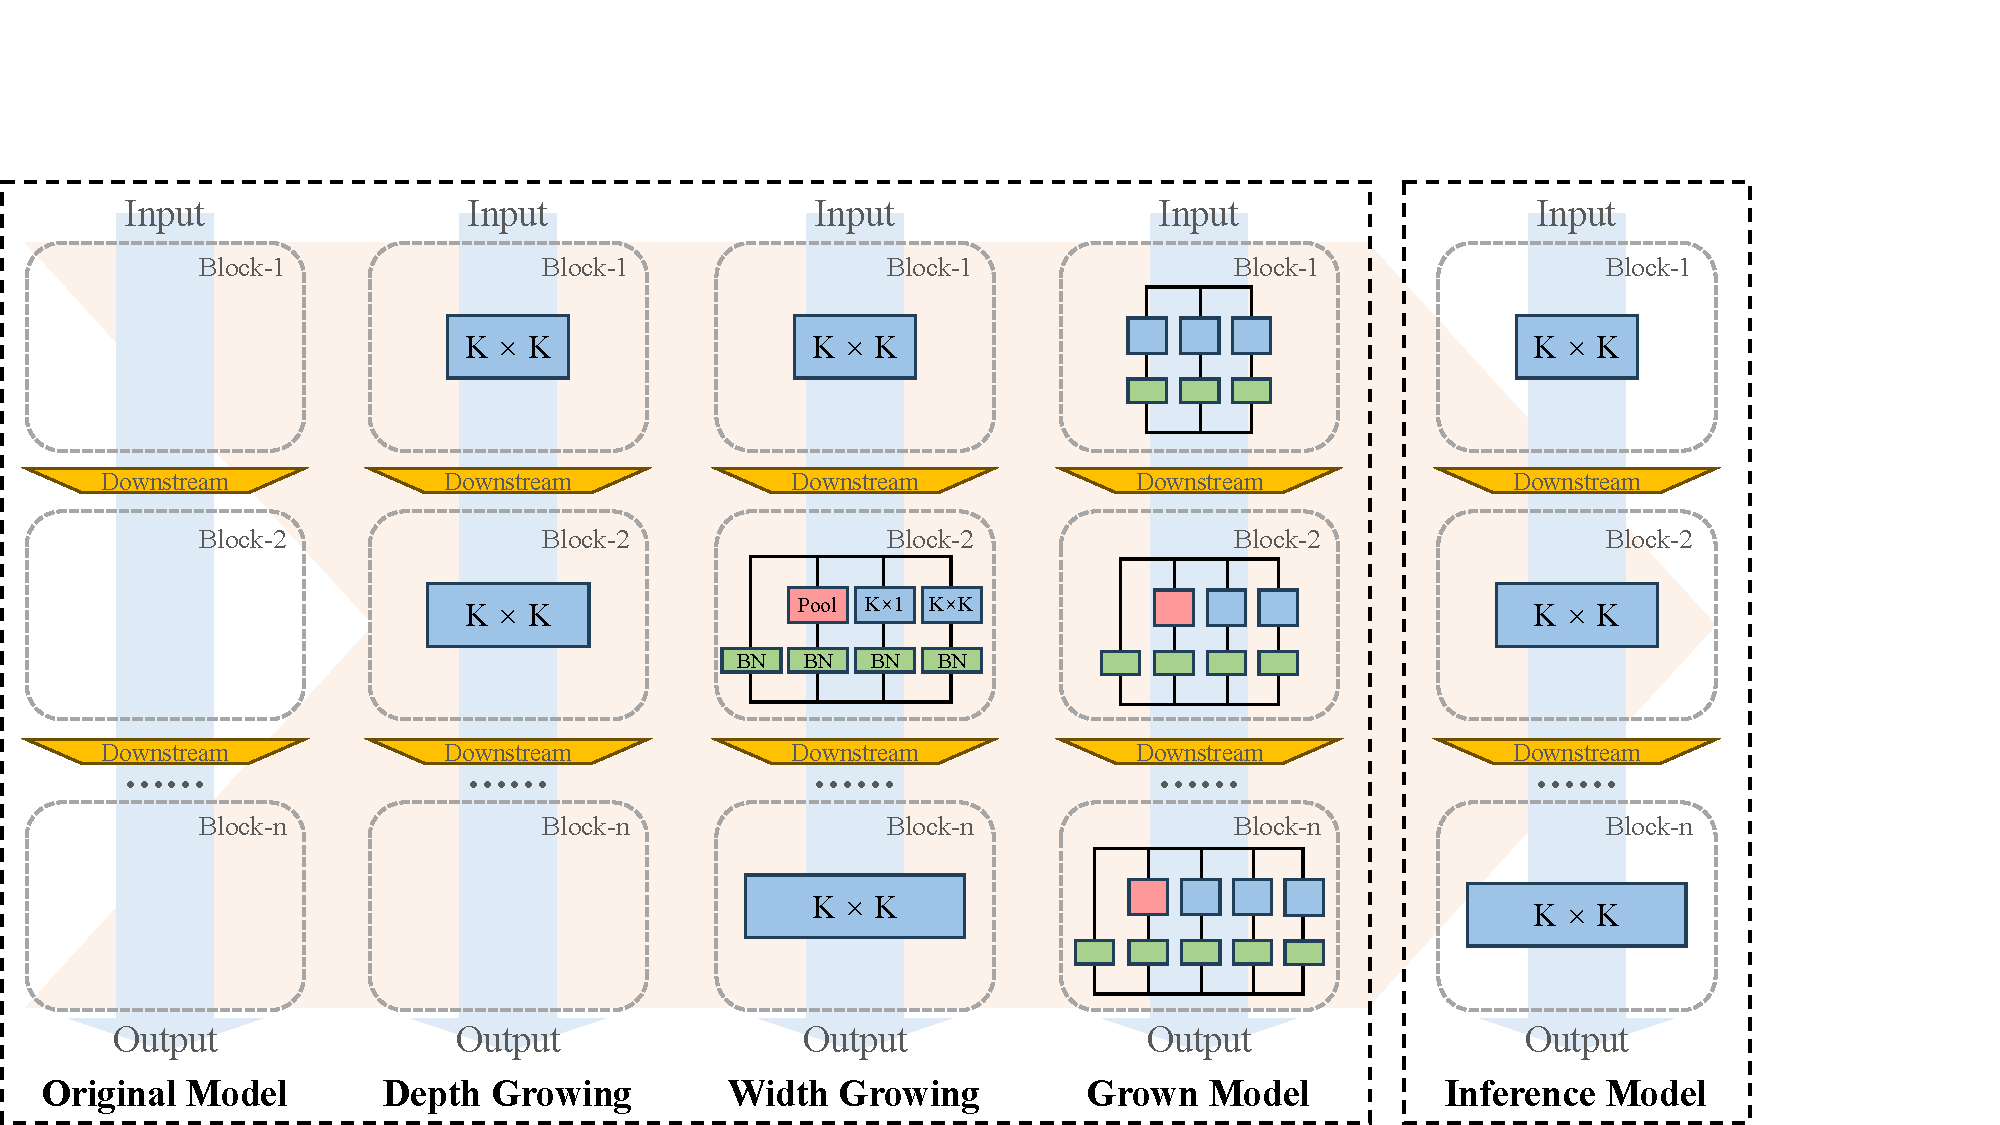
\includegraphics[width=\textwidth]{imgs/cnn.pdf}
  \caption{The process of the growing of convolutional neural networks.}
  \label{fig:cnn}
\end{figure*}

As shown in Figure \ref{fig:cnn}, our initial model is an "empty" model, containing only essential downsampling layers, drastically reducing parameter count and complexity. For example, the initial VGG model has only 169K parameters compared to 132M in a full VGG-11 model. This design lowers initial training costs and provides flexibility for growing.

Starting with this model, our framework systematically expands its depth and width. Depth expansion involves adding new layers to reserved computation blocks, depending on the architecture (see Table 3.1). Width expansion adds re-parameterizable branches to existing feature extraction structures, enhancing capability without increasing complexity. For instance, in the VGG architecture, a "Conv(64, 64, 1, 1)-BN(64)" module can be added in parallel to the "Conv(64, 64, 3, 3)-BN(64)" module, improving feature extraction with minimal training burden.

Proper initialization of new modules and adjustment of the optimizer are crucial for seamless integration. The grown network is streamlined through structural re-parameterization, resulting in a compact, efficient architecture that balances accuracy and inference efficiency, adapting well to specific task needs.

\subsubsection{Make Growing Decisions}

Model growing decision mechanism involves three key factors: the scale of single growing, the number of training iterations after growing, and the growing termination conditions. Using stochastic gradient descent (SGD) with a cosine learning rate schedule (initially set at 0.1), we conducted 100 growing training iterations on the CIFAR-10 dataset. To ensure experimental rigor, we fixed several strategies: inherited module initialization, inherited optimizer initialization, alternating width and depth growing, greedy growing location selection, and random width growing module selection. These will be discussed in detail later.

\textbf{Single growing scale}: We examined the impact of different scales in single growing iterations, both in depth and width. For depth growing, we fixed the post-growing training iterations at three and the growing endpoint at two sub-layers per computation block ("VGG-2-2-2" pattern). For width growing, we increased the width of 50\% of existing layers. Table \ref{table:single_depth_growth} shows performance differences when growing 1 to 6 layers in a single iteration.

\begin{table}[ht]
\centering
\tiny
\renewcommand{\arraystretch}{1.3}
\begin{adjustbox}{center}
\begin{tabular}{c|ccccccc}
\hline
\textbf{Depth Growing Scale} & \textbf{1 Layer} & \textbf{2 Layers} & \textbf{3 Layers} & \textbf{4 Layers} & \textbf{5 Layers} & \textbf{6 Layers} \\
\hline
\textbf{Architecture} & \multicolumn{6}{c}{VGG-2-2-2} \\
\hline
\textbf{\#Params} & \multicolumn{6}{c}{706.35K} \\
\hline
\textbf{FLOPs} & \multicolumn{6}{c}{161.38M} \\
\hline
\textbf{Acc\%} & 92.01 & 91.33 & 91.35 & 91.88 & 90.7 & 91.04 \\
\hline
\end{tabular}
\end{adjustbox}
\caption{Impact of Single Depth Growing Scale on Model Performance}
\label{table:single_depth_growth}
\end{table}

The experimental results show that the model performance is significantly affected by the number of layers added in each growing iteration. Adding only one layer at a time yields the best performance of 92.01\%, indicating that single-layer growing is the optimal strategy for depth expansion. Performance decreases with more layers, notably dropping to 90.7\% when five layers are added, due to the sudden increase in parameters and the instability caused by high learning rates during initial training.

Next, we analyze the impact of single-width growing on model performance. Unlike depth growing, width growing involves adding new re-parameterizable branches to one or more layers. Considering the limited parameter increase per branch, we examine proportional growing, such as expanding 50\% of existing layers. To ensure consistency, we use the optimal conclusions from prior experiments, such as single-layer depth growing. The impact of single-width growing scale on model performance is shown in Table \ref{table:single_width_growth}.

\begin{table}[ht]
\centering
\tiny
\renewcommand{\arraystretch}{1.3}
\begin{adjustbox}{center}
\begin{tabular}{c|ccccc}
\hline
\textbf{Width Growing Proportion} & \textbf{0\% (Depth Only)} & \textbf{30\%} & \textbf{50\%} & \textbf{70\%} & \textbf{100\% (All Layers)} \\
\hline
\textbf{Architecture} & \multicolumn{5}{c}{VGG-2-2-2} \\
\hline
\textbf{\#Params} & \multicolumn{5}{c}{706.35K} \\
\hline
\textbf{FLOPs} & \multicolumn{5}{c}{161.38M} \\
\hline
\textbf{Acc\%} & 90.88 & 92.05 & 92.01 & 92.42 & 92.09 \\
\hline
\end{tabular}
\end{adjustbox}
\caption{Impact of Single-Width Growing Scale on Model Performance}
\label{table:single_width_growth}
\end{table}

The results indicate that the scale of single-width growing affects performance. Compared to depth-only growing (90.88\%), the model performance increases to 92.05\% with 30\% width growing and further improves to 92.01\% and 92.42\% with 50\% and 70\% growing, respectively. However, performance slightly decreases to 92.09\% with 100\% growing, suggesting that while width growing enhances feature extraction, excessive growing may not be beneficial. Therefore, a balance is needed to optimize performance without overcomplicating the model.

\textbf{The frequency of training iterations after model growing} significantly impacts model performance. It ensures that the model has sufficient time to adjust and optimize the new structure, maximizing the potential performance improvement from each growing iteration. We examined the performance differences when the training iterations after growing ranged from 1 to 9 cycles, as shown in Table \ref{table:training_iterations}.

\begin{table}[ht]
\centering
\tiny
\renewcommand{\arraystretch}{1.3}
\begin{adjustbox}{center}
\begin{tabular}{c|ccccccc}
\hline
\textbf{Training Iterations} & \textbf{1} & \textbf{2} & \textbf{3} & \textbf{5} & \textbf{7} & \textbf{9} \\
\hline
\textbf{Architecture} & \multicolumn{6}{c}{VGG-2-2-2} \\
\hline
\textbf{\#Params} & \multicolumn{6}{c}{706.35K} \\
\hline
\textbf{FLOPs} & \multicolumn{6}{c}{161.38M} \\
\hline
\textbf{Acc\%} & 91.90 & 92.38 & 92.42 & 91.98 & 91.31 & 90.17 \\
\hline
\end{tabular}
\end{adjustbox}
\caption{Impact of Training Iterations After Growing on Model Performance}
\label{table:training_iterations}
\end{table}

The results indicate that the number of training iterations after growing affects model performance. Performance improves as iterations increase from 1 to 3, peaking at 92.42\% accuracy with 3 iterations. However, with more than 3 iterations, performance declines, likely due to overfitting and diminished returns from the new parameters. The optimization challenge can be described using the Taylor expansion of the loss function:

\begin{equation}
L(W^\ast + \Delta W) \approx L(W^\ast) + \nabla L(W^\ast)^T \Delta W + \frac{1}{2} \Delta W^T H \Delta W,
\end{equation}

where \( H \) is the Hessian matrix at \( W^\ast \). Since \( \nabla L(W^\ast)^T \approx 0 \) for well-trained \( W^\ast \), optimizing \( L(W^\ast + \Delta W) \) tends to drive \( \Delta W \) towards zero, contributing little to performance improvement. Thus, excessive training iterations after growing may lead to performance decline due to optimization inefficiency.

\textbf{Model Growing Termination Conditions}: Setting appropriate termination conditions for model growing is crucial for achieving optimal performance, inference efficiency, and practical application value. We offer diverse termination conditions to accommodate users from different backgrounds.

For architecture experts, the framework allows precise customization of the final model architecture, such as "VGG-2-2-2-2" or "ResNet-3-4-5-3". This approach ensures the model development aligns with expert expectations. Advanced designs like Swin Transformer and ConvNeXt have used patterns like "2-2-18-2" and "3-3-27-3", emphasizing key transition blocks for high-level feature extraction.

For application experts who may not be familiar with architectural details but have performance expectations, we provide a parameter-based termination condition. Users can set a maximum parameter limit post-reparameterization (e.g., 20M). To prevent excessive width expansion, the pre-reparameterization parameter count must not exceed 1.5 times the set limit. This flexibility allows for either a shallow, wide model with lower inference costs or a deep, narrow model with potential higher performance.

For other domain experts, an automatic growing termination mechanism is available. It stops growing when performance gains plateau, based on an exponential moving average (EMA) \cite{ema} of model accuracy. If performance improvement falls below a user-defined threshold (default 3\%) for several iterations, growing is terminated. This approach balances performance optimization and training stability.

Table \ref{table:termination_conditions} shows the impact of different termination conditions on model performance and efficiency.

\begin{table}[ht]
\centering
\tiny
\renewcommand{\arraystretch}{1.3}
\begin{adjustbox}{center}
\begin{tabular}{c|ccccc}
\hline
\textbf{Termination Condition} & \textbf{Architecture} & \textbf{Parameter} & \textbf{Auto} & \textbf{Auto} & \textbf{Auto} \\
\hline
\textbf{Control Condition} & VGG-3-3-3 & 1M & Default & Threshold 6\% & Tolerance 3\ \\
\hline
\textbf{Post-Growing Arch} & VGG-3-3-3 & VGG-4-3-3 & VGG-2-3-2 & VGG-1-2-2 & VGG-3-4-3 \\
\hline
\textbf{\#Params} & 974.47K & 1.01M & 789.58K & 669.29K & 1.06M \\
\hline
\textbf{FLOPs} & 230.20M & 268.21M & 182.72M & 123.37M & 251.53M \\
\hline
\textbf{Acc\%} & 93.01 & 92.74 & 92.14 & 92.08 & 92.57 \\
\hline
\end{tabular}
\end{adjustbox}
\caption{Impact of Termination Conditions on Model Growing}
\label{table:termination_conditions}
\end{table}

Our framework's flexible termination conditions cater to various users, ensuring optimal model performance and efficiency tailored to different needs. This design enhances the framework's adaptability and provides a robust foundation for efficient model growing.

\subsubsection{Network Module Selection and Growing}

During the model's growing process, the selection of network modules and growing strategies is crucial for optimizing performance and improving computational efficiency.

\textbf{Depth Growing Decision Scheme}: The strategy for depth growing significantly impacts the final performance and efficiency of growing models. For anisotropic convolutional neural networks, the layer configuration within each computational block is consistent, while it varies between blocks. Therefore, the focus is on determining the optimal growing location, both at the block level and within the block. This section explores the decision process to optimize model structure and enhance performance.

We investigated three main growing location decision methods: random selection, sequential selection, and an innovative greedy selection. Random selection arbitrarily determines the block and position for layer growing. Sequential selection adds new layers to the end of each selected block in a fixed order. Greedy selection, based on the network's dynamic importance \cite{bnpruning} during training, prioritizes adding depth to the most important block and position. This importance is quantified by analyzing inherent scaling behaviors, such as the weights of batch normalization layers, which reflect the importance of output feature maps, as shown in Figure \ref{fig:saliency}.

\begin{figure*}
  \centering
  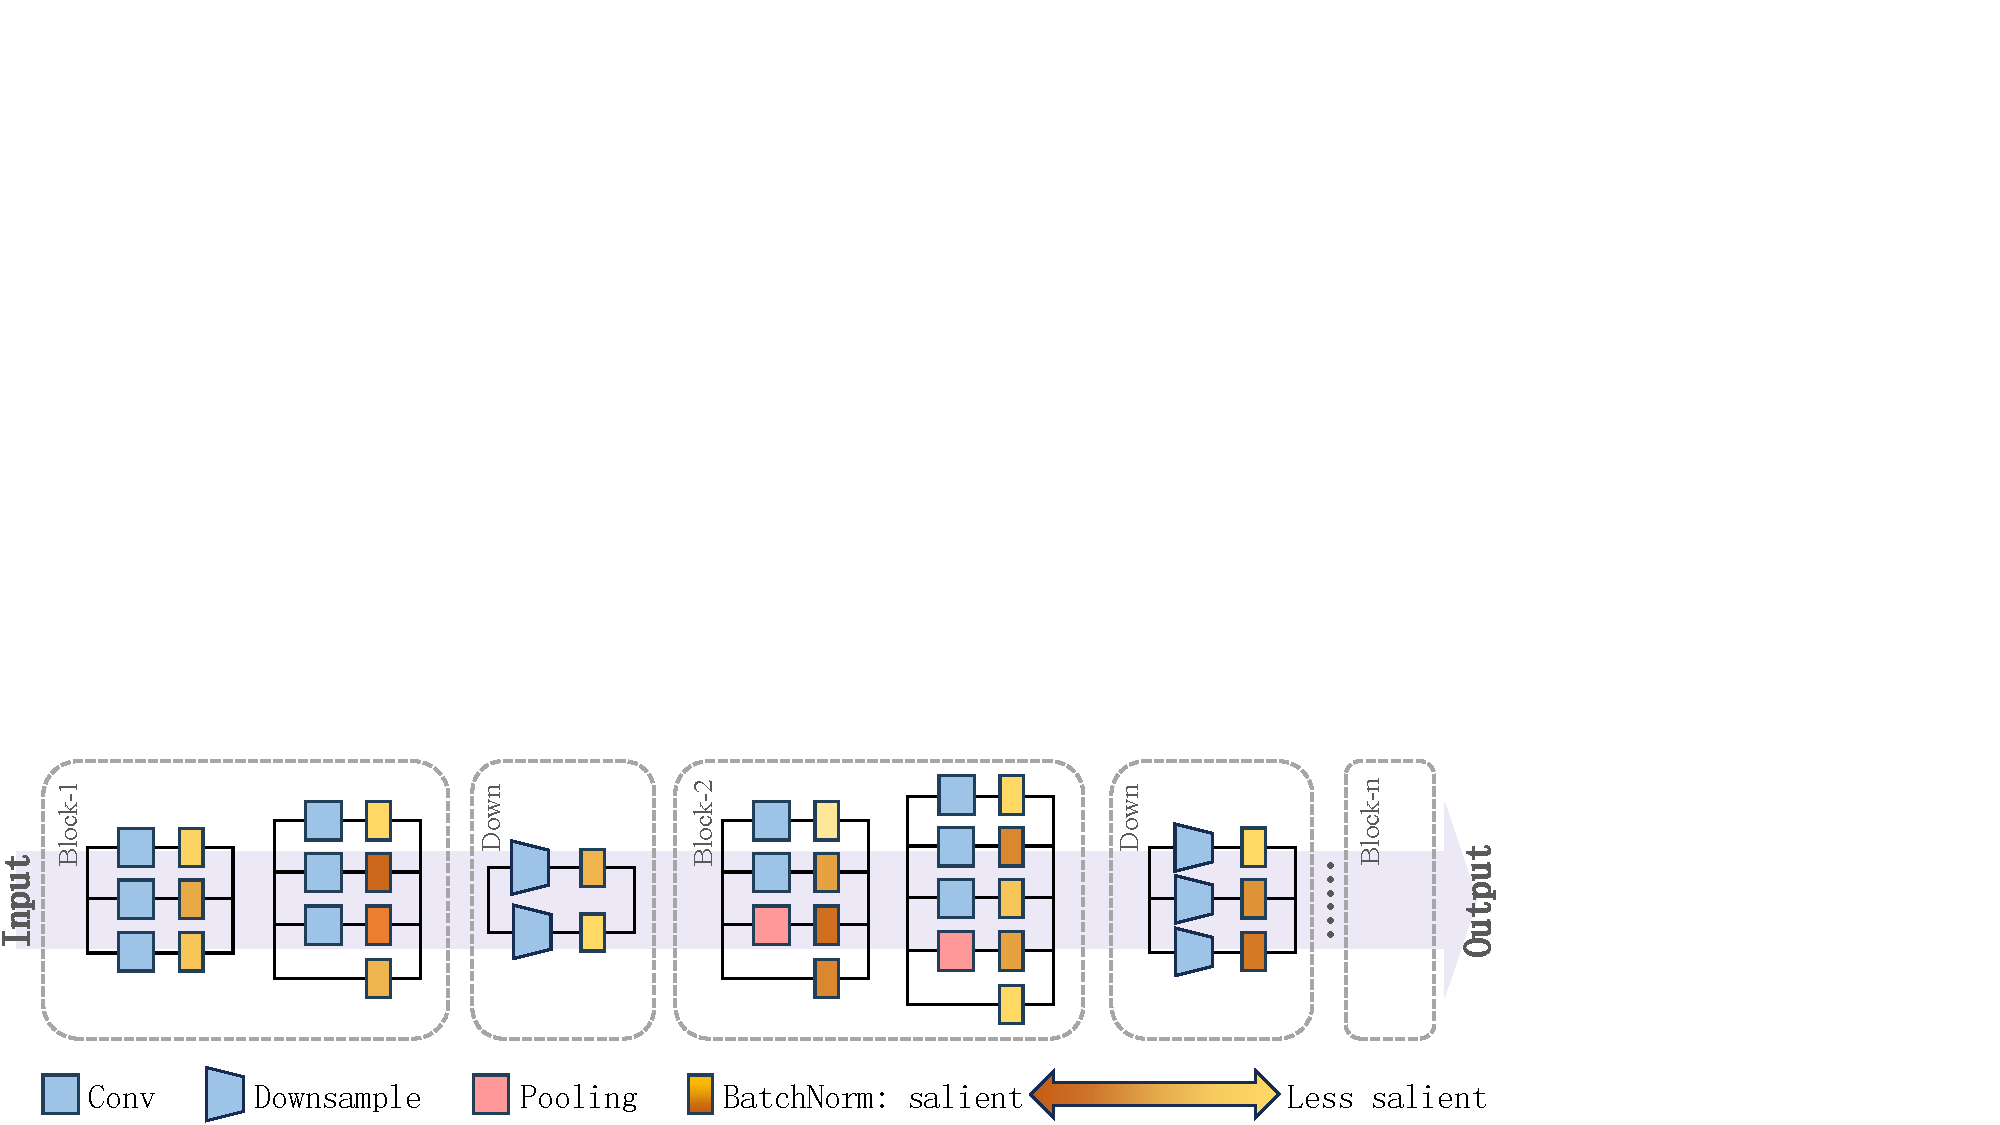
\includegraphics[width=\textwidth]{imgs/saliency.pdf}
  \caption{The importance of pre-existing scaling in neural networks.}
  \label{fig:saliency}
\end{figure*}

For the greedy selection strategy, we first collect the scaling weights of batch normalization layers outside all computational blocks. For layers in parallel branches, we average the scaling weights to reflect each block's importance. During depth growing decisions, these absolute scaling factors serve as the standard for importance, prioritizing the block with the highest absolute scaling factor for depth expansion. Subsequently, the most important layer within the selected block is identified for growing. Table \ref{table:depth_growth_strategies} compares the performance of greedy selection with random and sequential selection strategies under optimal conditions.

\begin{table}[ht]
\centering
\tiny
\renewcommand{\arraystretch}{1.3}
\begin{adjustbox}{center}
\begin{tabular}{c|ccc}
\hline
\textbf{Depth Growing Strategy} & \textbf{Random Selection} & \textbf{Sequential Selection} & \textbf{Greedy Selection} \\
\hline
\textbf{Architecture} & \multicolumn{3}{c}{VGG-2-2-2} \\
\hline
\textbf{\#Params} & \multicolumn{3}{c}{706.35K} \\
\hline
\textbf{FLOPs} & \multicolumn{3}{c}{161.38M} \\
\hline
\textbf{Acc\%} & 92.07 & 92.16 & 92.42 \\
\hline
\end{tabular}
\end{adjustbox}
\caption{Impact of Depth Growing Strategies on Model Performance}
\label{table:depth_growth_strategies}
\end{table}

The results indicate that different depth growing strategies impact model performance. The greedy selection strategy achieved the highest accuracy of 92.42\%, outperforming random and sequential strategies by 0.35\% and 0.26\%, respectively. This validates the effectiveness of growing modules at important expression positions in the model. The importance-based scaling factor analysis provides a clear path for dynamic model structure optimization.

\textbf{Width Growing Decision Scheme}: In the growing process of models, width growing is crucial for enhancing the model's ability to extract diverse features. Instead of actual width increase, we adopt a structural re-parameterization-based simulated width growing to maintain high inference efficiency while improving feature extraction. This section explores which layers need width growing and how to implement it effectively.

Following the proven effectiveness of the greedy selection mechanism for depth growing, we apply this approach to width growing. We evaluate the importance scaling factors of all layers, including downsampling layers, to capture the contribution differences to final performance. We select the top 70\% of layers based on importance for width growing.

Once the candidate layers for width growing are identified, the next step is to determine how to enhance feature extraction by adding re-parameterizable branches. Using the maximum receptive field of the original single-branch layer as a baseline, we introduce various sub-receptive field sizes and common re-parameterizable branches such as average pooling and independent batch normalization layers, forming a diverse branch search space, as shown in Figure \ref{fig:branches}. This process maintains re-parameterization principles for efficiency and introduces functional diversity.

\begin{figure*}
  \centering
  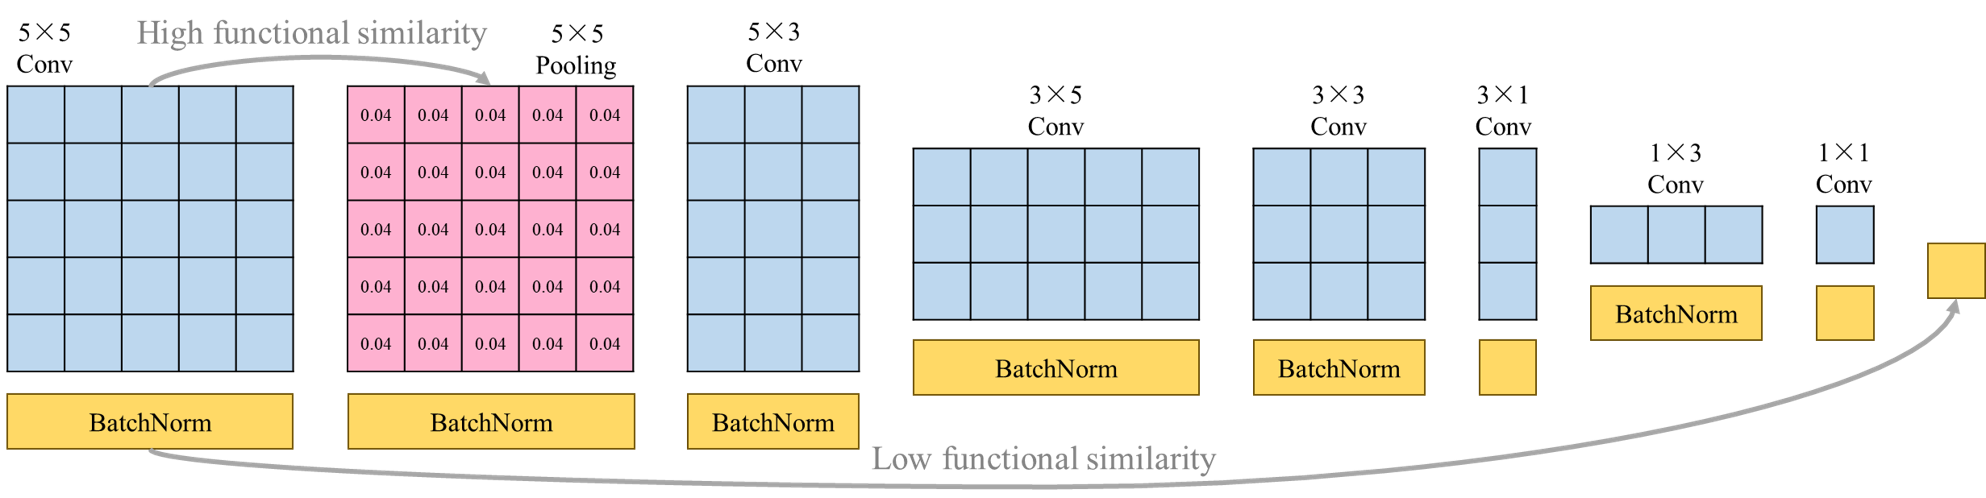
\includegraphics[width=\textwidth]{imgs/branches.png}
  \caption{Search space for branches to be inserted in width growing.}
  \label{fig:branches}
\end{figure*}

When a layer meets the width growing criteria, a branch from the search space is selected and inserted. We examined three branch selection strategies: without-replacement random sampling, with-replacement random sampling, and without-replacement greedy sampling.

Without-replacement greedy sampling follows a "maximum differentiation" principle: selecting branches that differ the most from existing ones to enhance diverse feature extraction. We rank all branches based on functional similarity, then select and remove the most optimal branch from the ordered set until it is empty. For instance, in Figure 3.5, a possible selection order for greedy sampling is: [independent normalization layer, 3×3 convolution layer, 5×3 convolution layer, 1×3 convolution layer, 5×5 pooling layer, 3×5 convolution layer, 3×1 convolution layer, 1×1 convolution layer]. This method limits the width growing to the full branch search space.

Without-replacement random sampling aims to cover the search space fully, while with-replacement random sampling has no upper limit, providing higher flexibility. Table \ref{table:width_growth_branches} compares the performance impact of different branch selection methods under optimal conditions.

\begin{table}[ht]
\centering
\tiny
\renewcommand{\arraystretch}{1.3}
\begin{adjustbox}{center}
\begin{tabular}{c|ccc}
\hline
\textbf{Branch Selection Method} & \textbf{W/o replacement Rand} & \textbf{W replacement Rand} & \textbf{W/o replacement Greedy} \\
\hline
\textbf{Architecture} & \multicolumn{3}{c}{VGG-2-2-2} \\
\hline
\textbf{\#Params} & \multicolumn{3}{c}{706.35K} \\
\hline
\textbf{FLOPs} & \multicolumn{3}{c}{161.38M} \\
\hline
\textbf{Acc\%} & 91.93 & 92.42 & 92.11 \\
\hline
\end{tabular}
\end{adjustbox}
\caption{Impact of Branch Selection Methods on Model Performance in Width Growing}
\label{table:width_growth_branches}
\end{table}

The results show that the branch selection method significantly impacts model performance. With-replacement random sampling achieved the highest accuracy at 92.42\%, outperforming without-replacement random sampling (91.93\%) and greedy sampling (92.11\%). This suggests that the flexibility of with-replacement random sampling, allowing multiple selections of the same branch, provides better performance. Greedy sampling outperformed random sampling without replacement, validating its effectiveness in enhancing feature diversity, making it a practical method for efficient branch selection.

\textbf{Coordinating Depth and Width Growing}: The next phase of model structure optimization involves exploring the optimal balance between depth and width growing. Properly balancing these growing proportions is crucial for enhancing overall performance, feature extraction capabilities, and inference efficiency. We analyzed different growing proportion strategies, such as "one width growing for every two depth growing" and "two width growing for every depth growing," to identify which strategy offers the most potential for performance improvement. Table \ref{table:depth_width_matching} presents the experimental results under optimal conditions.

\begin{table}[ht]
\centering
\tiny
\renewcommand{\arraystretch}{1.3}
\begin{adjustbox}{center}
\begin{tabular}{c|ccccc}
\hline
\textbf{Growing Matching Method} & \textbf{Width 3, Depth 1} & \textbf{Width 2, Depth 1} & \textbf{Width 1, Depth 1} & \textbf{Width 1, Depth 2} & \textbf{Width 1, Depth 3} \\
\hline
\textbf{Architecture} & \multicolumn{5}{c}{VGG-4-4-4} \\
\hline
\textbf{\#Params} & \multicolumn{5}{c}{1.24M} \\
\hline
\textbf{FLOPs} & \multicolumn{5}{c}{299.01M} \\
\hline
\textbf{Acc\%} & 93.40 & 93.91 & 93.85 & 94.36 & 93.78 \\
\hline
\end{tabular}
\end{adjustbox}
\caption{Impact of Coordinating Depth and Width Growing on Model Performance}
\label{table:depth_width_matching}
\end{table}

The results indicate that different coordination strategies of width and depth growing affect model performance. Among these strategies, the "one width growing for every two depth growing" method achieved the best accuracy of 94.36\%, significantly outperforming other ratios. This suggests that a moderate bias towards depth growing over width growing more effectively enhances model performance, consistent with our experience that deeper neural networks tend to improve performance. Therefore, we recommend a depth-priority growing strategy when designing high-performance model structures to ensure optimal performance while maintaining computational efficiency.

\subsubsection{Initialize New Parameters and Optimizers}

As the model grows, initializing newly added network modules and adjusting the corresponding optimizer are crucial for ensuring steady performance improvement. This section explores how to select the best initialization method for new modules to achieve rapid model convergence and how to adjust or update the optimizer to accommodate changes in network structure. These steps ensure that new structures integrate smoothly with the existing model without compromising learning efficiency. Figure \ref{fig:ini} illustrates the initialization and optimizer adjustment requirements brought about by new modules.

\begin{figure*}
  \centering
  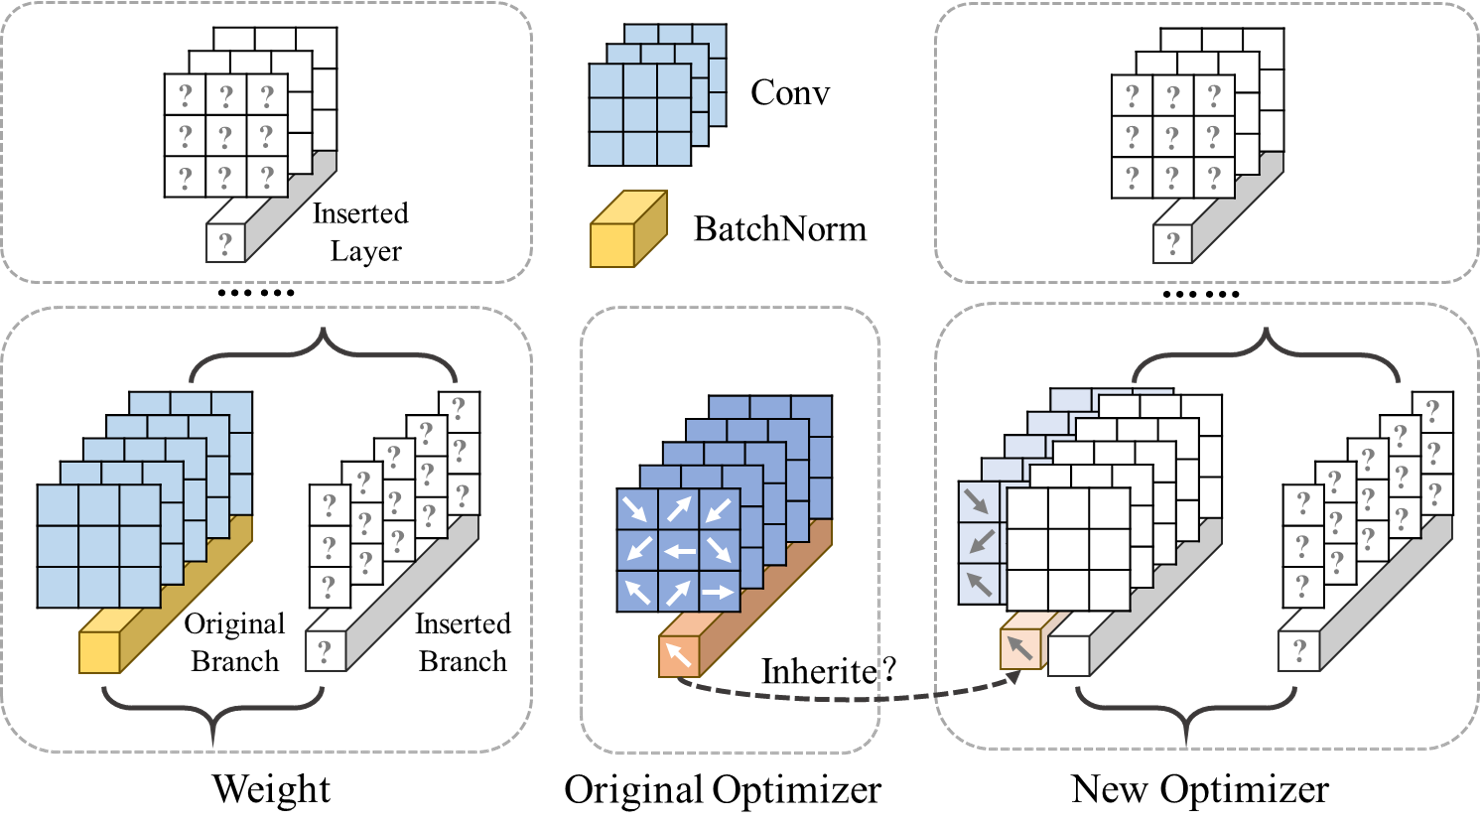
\includegraphics[width=0.85\textwidth]{imgs/ini.png}
  \caption{Search space for branches to be inserted in width growing.}
  \label{fig:ini}
\end{figure*}

\textbf{Parameter Initialization Strategy for New Modules}: This study considers various initialization methods for new modules, including zero initialization, inherited initialization, uniform distribution initialization, Gaussian distribution initialization, Gaussian local fitting initialization, Gaussian global fitting initialization, and a local learning-based initialization method.

Inherited initialization maintains consistency by using the same initialization method for new modules as existing ones in the original model (e.g., Kaiming initialization for convolution weights and zero initialization for biases). Gaussian local and global fitting initialization set new module parameters based on statistical analysis of existing modules (local: neighbors; global: all modules). The local learning initialization method optimizes new modules separately with a low learning rate (1e-3) before integrating them into the full model, maximizing their potential and improving overall network performance.

\begin{table}[ht]
\centering
\tiny
\renewcommand{\arraystretch}{1.3}
\begin{adjustbox}{center}
\begin{tabular}{c|c|c|c|c|c}
\hline
\textbf{Initialization Method} & \textbf{Configuration} & \textbf{Grown Arch} & \textbf{Params} & \textbf{FLOPs} & \textbf{Acc\%} \\
\hline
Zero Initialization & - & \multirow{11}{*}{VGG-2-2-2} & \multirow{11}{*}{706.35K} & \multirow{11}{*}{161.38M} & 40.16 \\
Uniform Distribution Initialization & [-0.01, 0.01] & & & & 91.00 \\
Uniform Distribution Initialization & [-0.1, 0.1] & & & & 91.56 \\
Uniform Distribution Initialization & [-0.3, 0.3] & & & & 91.80 \\
Gaussian Distribution Initialization & $\mu=0$; $\sigma=0.01$ & & & & 91.56 \\
Gaussian Distribution Initialization & $\mu=0$; $\sigma=0.1$ & & & & 91.34 \\
Gaussian Distribution Initialization & $\mu=0$; $\sigma=0.3$ & & & & 91.28 \\
Gaussian Local Fitting Initialization & - & & & & 91.27 \\
Gaussian Global Fitting Initialization & - & & & & 91.71 \\
Local Learning Initialization & Adam & & & & 90.68 \\
Inherited Initialization & - & & & & 92.42 \\
\hline
\end{tabular}
\end{adjustbox}
\caption{Impact of Initialization Methods on Model Growing Performance}
\label{table:initialization_methods}
\end{table}


Table \ref{table:initialization_methods} indicate that inherited initialization achieved the highest accuracy at 92.42\%, demonstrating the importance of maintaining initialization consistency with the original model. Zero initialization significantly dropped performance to 40.16\%, highlighting its detrimental effect due to disrupting weight asymmetry, causing new neurons to update similarly and losing network diversity. Uniform and Gaussian distribution initializations showed varying performance based on hyperparameter settings, with uniform initialization in the [-0.3, 0.3] range achieving 91.80\% accuracy, slightly outperforming Gaussian initialization. Local and global Gaussian fitting initializations achieved 90.68\% and 91.27\%, respectively, potentially limiting new module potential by relying too heavily on existing parameter distributions. Local learning initialization showed a relatively high accuracy of 91.71\%, indicating the effectiveness of targeted new module optimization. Overall, inherited initialization was the most effective, ensuring training stability and performance improvement during model growing.

\textbf{Optimizer Adjustment Strategy}: As the model grows and new parameters are introduced, managing the optimizer's state \cite{optimizer} and adaptability becomes critical for training efficiency and performance optimization. A key issue in constructing a new optimizer is whether to inherit state information from the old optimizer. This state often includes first and second-order momentum information, learning rate schedules, etc., which are crucial for optimization stability and convergence speed. This study experimentally verifies the impact of inheriting the old optimizer's state when creating a new optimizer for the grown model. Table \ref{table:optimizer_adjustment} compares the performance and training efficiency of a fresh optimizer versus an inherited state optimizer under optimal conditions.

\begin{table}[ht]
\centering
\tiny
\renewcommand{\arraystretch}{1.3}
\begin{adjustbox}{center}
\begin{tabular}{c|ccccc}
\hline
\textbf{Optimizer Adjustment Strategy} & \textbf{New Optimizer} & \textbf{Inherited Optimizer State} \\
\hline
Grown Arch & \multicolumn{2}{c}{VGG-2-2-2} \\
\hline
Params & \multicolumn{2}{c}{706.35K} \\
\hline
FLOPs & \multicolumn{2}{c}{161.38M} \\
\hline
Acc\% & 92.21 & 92.42 \\
\hline
\end{tabular}
\end{adjustbox}
\caption{Impact of Optimizer Adjustment Strategies on Model Growing Performance}
\label{table:optimizer_adjustment}
\end{table}

The results show that the inherited state optimizer strategy achieved an accuracy of 92.42\%, outperforming the new optimizer strategy, which achieved 92.21\%. This indicates that inheriting the optimizer's state is crucial for maintaining training continuity and accelerating convergence. While a new optimizer offers a clean slate, it lacks historical training context, potentially requiring more time to adjust and optimize the new parameters. In contrast, the inherited optimizer can quickly adapt to structural changes by retaining momentum and other state information, leading to more efficient parameter updates and faster performance improvement. Therefore, this study recommends prioritizing the inherited optimizer strategy during model structure adjustments to leverage the accumulated optimization state and enhance model performance effectively.

\subsection{Experimental Validation on Model Growing}

\subsubsection{Introduction to the Dataset and Experimental Configuration}

To validate whether the proposed model growing framework can train neural networks that are both high-performing and efficient with good task adaptability, we further conduct performance and efficiency verification analysis on various convolutional neural network models (specifically VGG, ResNet, ResNet-Bottleneck, and MobileNetV3) across different datasets. The datasets used in this study are introduced in Table \ref{table:datasets}.

\begin{table}[ht]
\centering
\tiny
\renewcommand{\arraystretch}{1.3}
\begin{adjustbox}{center}
\begin{tabular}{c|p{10cm}}
\hline
\textbf{Dataset} & \textbf{Description} \\
\hline
CIFAR10 \cite{cifar} & Contains 60,000 32×32 color images in 10 classes, with 6,000 images per class. There are 50,000 training images and 10,000 test images. CIFAR-10 is used for low-resolution visual tasks without fine-grained recognition. \\
\hline
CIFAR100 \cite{cifar} & A fine-grained version of CIFAR10, containing 100 classes with 600 images per class. It has lower resolution and a smaller dataset size. \\
\hline
SVHN \cite{svhn} & Street View House Numbers for digit recognition, containing 73,257 training images and 26,032 test images, all at 32×32 resolution. It is a low-resolution dataset without fine-grained recognition. \\
\hline
MNIST \cite{mnist} & A classic handwritten digit recognition dataset with 60,000 training images and 10,000 test images, all at 28×28 resolution in grayscale. It is a low-resolution, non-fine-grained dataset. \\
\hline
ImageWoof \cite{imagenet} & Fine-grained dog breed recognition with 9,025 training and 3,929 validation images at 224×224 resolution across 10 classes. \\
\hline
ImagenetTE \cite{imagenet} & High-resolution easy classification images at 224×224 resolution, with 9,649 training and 3,925 validation images across 10 classes. \\
\hline
Tiny-Imagenet \cite{imagenet} & Contains 200 classes with 500 training, 50 validation, and 50 test images per class at 64×64 resolution. It is a high-challenge, compact dataset. \\
\hline
Mini-Imagenet \cite{imagenet} & Contains 100 classes with 48,000 training and 12,000 validation samples at 224×224 resolution. \\
\hline
\end{tabular}
\end{adjustbox}
\caption{Introduction of Datasets Involved in the Experiments}
\label{table:datasets}
\end{table}

Based on the optimization of the growing strategy explored in the previous sections, the configurations for the growing of neural networks are shown in Table \ref{table:growth_configuration}.

\begin{table}[ht]
\centering
\tiny
\renewcommand{\arraystretch}{1.3}
\begin{adjustbox}{center}
\begin{tabular}{c|p{10cm}}
\hline
\textbf{Configuration Item} & \textbf{Configuration Details} \\
\hline
Global Configuration & Initial learning rate of 0.1 for growing; cosine-based learning rate adjustment; SGD optimizer; experimental framework in PyTorch \cite{pytorch}; efficiency testing on NVIDIA A100 PCIE 40GB GPU; fixed-scale models using architectures from Huggingface/Timm; Adam optimizer with an initial learning rate of 5e-3; cosine-based learning rate adjustment; second-order weight regularization with a strength of 5e-4. \\
\hline
Special Configuration & Due to the simplicity of the MNIST dataset, manual control limits each computation block to a maximum of one layer before stopping; other datasets use automatic growing termination. \\
\hline
Fix-sized Models & Total training epochs: 100; inherited initialization for new parameters; inherited optimizer adjustment; single training iteration after adding new modules: 3 epochs; greedy selection for growing location; random sampling with replacement for width growing re-parameterizable branches; growing ratio of one width to two depths. \\
\hline
\end{tabular}
\end{adjustbox}
\caption{Model Growing Configuration Scheme}
\label{table:growth_configuration}
\end{table}

These configurations are designed to ensure the model grows effectively and efficiently while adapting to various tasks, thereby validating the robustness and flexibility of the proposed model growing framework.

\subsubsection{Task Adaptation Evaluation}

To evaluate the adaptability of growing convolutional neural networks across different tasks, this study selected a diverse range of datasets including CIFAR-10, CIFAR-100, SVHN, MNIST, ImagenetTE, ImageWoof, Tiny-ImageNet, and Mini-ImageNet. These tasks cover a spectrum from simple to complex ones, low to high resolution, non-fine-grained to fine-grained recognition, and single to multi-channel image recognition. The chosen baselines for comparison are a series of fixed-scale classic models, including ResNet (both standard and Bottleneck architectures), VGG, and MobileNetV3.

\begin{table}[ht]
\centering
\tiny
\renewcommand{\arraystretch}{1.3}
\begin{adjustbox}{center}
\begin{tabular}{lccccc}
\hline
\textbf{Model} & \textbf{Arch} & \textbf{Params} & \textbf{FLOPs} & \textbf{Latency(ms)} & \textbf{Acc\%} \\
\hline
ResNet-18 & 2-2-2-2 & 11.69M & 558.39M & 3.83 & 87.76 \\
ResNet-34 & 3-4-6-3 & 21.80M & 1.16G & 6.92 & 87.60 \\
ResNet-50(bottleneck) & 3-4-6-3 & 25.56M & 1.31G & 9.25 & 86.12 \\
ResNet-101(bottleneck) & 3-4-23-3 & 44.55M & 2.53G & 17.87 & 86.02 \\
growing ResNet & 1-2-2 & 1.17M & 222.99M & 1.90 & 92.22 \\
growing ResNet & 1-2-2-1 & 2.65M & 246.66M & 2.11 & 93.14 \\
growing Bottleneck-ResNet & 2-2-2 & 235.07K & 41.09M & 2.18 & 90.08 \\
growing Bottleneck-ResNet & 2-2-2-2 & 673.21K & 48.14M & 2.89 & 90.94 \\ \hline
VGG-11 & 1-1-2-2-2 & 140.72M & 440.32M & 3.14 & 89.17 \\
VGG-16 & 2-2-3-3-3 & 146.22M & 601.25M & 3.26 & 90.48 \\
growing VGG & 1-2-2 & 669.29K & 123.37M & 1.08 & 90.72 \\
growing VGG & 1-1-2-2 & 2.06M & 125.72M & 1.37 & 91.44 \\ \hline
MobileNetV3-small & 2-2-3-2-2 & 2.84M & 8.98M & 7.64 & 65.84 \\
MobileNetV3-large & 2-2-3-4-2-2 & 5.74M & 17.78M & 16.98 & 70.32 \\
growing MobileNetV3 & 2-3-3 & 811.40K & 20.37M & 3.71 & 89.32 \\
growing MobileNetV3 & 2-2-3-2 & 670.52K & 7.24M & 4.40 & 88.31 \\
\hline
\end{tabular}
\end{adjustbox}
\caption{Impact of growing on Convolutional Neural Networks for CIFAR-10}
\label{table:cifar10_self_growth}
\end{table}

Table \ref{table:cifar10_self_growth} demonstrates the performance of the growing convolutional neural network versus the fixed-scale network on the CIFAR-10 dataset. The growing model achieves a huge accuracy improvement with superb overall efficiency, and this improvement is even more obvious on the performance-biased MobileNetV3 family of models, demonstrating the advantages of the growing strategy in model optimization and task adaptation improvement.

\begin{table}[ht]
\centering
\tiny
\renewcommand{\arraystretch}{1.3}
\begin{adjustbox}{center}
\begin{tabular}{lccccc}
\hline
\textbf{Model} & \textbf{Arch} & \textbf{Params} & \textbf{FLOPs} & \textbf{Latency(ms)} & \textbf{Acc\%} \\
\hline
ResNet-18 & 2-2-2-2 & 11.69M & 558.39M & 3.83 & 55.80 \\
ResNet-34 & 3-4-6-3 & 21.80M & 1.16G & 6.92 & 55.40 \\
ResNet-50(bottleneck) & 3-4-6-3 & 25.56M & 1.31G & 9.25 & 53.16 \\
ResNet-101(bottleneck) & 3-4-23-3 & 44.55M & 2.53G & 17.87 & 53.40 \\
growing ResNet & 2-2-2 & 1.24M & 299.01M & 1.88 & 70.64 \\
growing ResNet & 1-2-2-2 & 3.83M & 265.57M & 2.43 & 72.90 \\
growing Bottleneck-ResNet & 2-3-3 & 262.99K & 44.91M & 2.54 & 67.52 \\
growing Bottleneck-ResNet & 2-2-3-2 & 691.03K & 49.30M & 3.39 & 69.78 \\ \hline
VGG-11 & 1-1-2-2-2 & 140.72M & 440.32M & 3.14 & 59.27 \\
VGG-16 & 2-2-3-3-3 & 146.22M & 601.25M & 3.26 & 59.32 \\
growing VGG & 2-3-3 & 937.42K & 192.19M & 1.40 & 67.84 \\
growing VGG & 2-2-3-2 & 2.33M & 194.53M & 1.79 & 69.46 \\ \hline
MobileNetV3-small & 2-2-3-2-2 & 2.84M & 8.98M & 7.64 & 34.04 \\
MobileNetV3-large & 2-2-3-4-2-2 & 5.74M & 17.78M & 16.98 & 33.80 \\
growing MobileNetV3 & 3-4-3 & 903.18K & 25.80M & 4.97 & 66.54 \\
growing MobileNetV3 & 3-3-3-3 & 855.29K & 9.33M & 5.73 & 63.82 \\
\hline
\end{tabular}
\end{adjustbox}
\caption{Growing Effects on Convolutional Neural Networks for CIFAR-100}
\label{table:cifar100_self_growth}
\end{table}

Table \ref{table:cifar100_self_growth} shows the results of comparing the performance of growing convolutional neural networks with fixed-architecture models on the CIFAR-100 dataset, where the growing approach once again demonstrates its superior ability in terms of task adaptability, while achieving a balance between performance and efficiency. In particular, for the MobileNetV3 family of models, which are difficult to cope with the CIFAR-100 dataset, the growing model improves its performance by about double (from 33.04\% to 66.54\%).CIFAR-100 is a fine-grained version of CIFAR-10, which, in contrast, has a larger number of total categories, less data for individual categories, and a higher overall difficulty level, and thus the self growing model will ultimately exceed the size of the CIFAR-10 dataset, reflecting the strength of the growing approach's ability to analyze specific tasks specifically. Even so, the growing model still has a higher inference efficiency than the fixed-size model in terms of the number of parameters, the amount of computation, and the inference latency.

\begin{table}[ht]
\centering
\tiny
\renewcommand{\arraystretch}{1.3}
\begin{adjustbox}{center}
\begin{tabular}{lccccc}
\hline
\textbf{Model} & \textbf{Arch} & \textbf{Params} & \textbf{FLOPs} & \textbf{Latency (ms)} & \textbf{Acc\%} \\
\hline
ResNet-18 & 2-2-2-2 & 11.69M & 558.39M & 3.83 & 95.07 \\
ResNet-34 & 3-4-6-3 & 21.80M & 1.16G & 6.92 & 95.41 \\
ResNet-50(bottleneck) & 3-4-6-3 & 25.56M & 1.31G & 9.25 & 96.13 \\
ResNet-101(bottleneck) & 3-4-23-3 & 44.55M & 2.53G & 17.87 & 96.57 \\
growing ResNet & 1-1-1 & 706.35K & 161.38M & 1.17 & 96.01 \\
growing ResNet & 1-2-1-1 & 2.35M & 227.72M & 1.82 & 96.55 \\
growing Bottleneck-ResNet & 1-2-1 & 212.68K & 35.08M & 1.52 & 95.56 \\
growing Bottleneck-ResNet & 1-1-2-1 & 588.08K & 39.50M & 1.99 & 96.21 \\ \hline
VGG-11 & 1-1-2-2-2 & 140.72M & 440.32M & 3.14 & 95.76 \\
VGG-16 & 2-2-3-3-3 & 146.22M & 601.25M & 3.26 & 95.91 \\
growing VGG & 1-2-1 & 521.45K & 113.90M & 1.03 & 95.87 \\
growing VGG & 1-1-2-1 & 1.47M & 116.26M & 1.21 & 95.80 \\ \hline
MobileNetV3-small & 2-2-3-2-2 & 2.84M & 8.98M & 7.64 & 92.26 \\
MobileNetV3-large & 2-2-3-4-2-2 & 5.74M & 17.78M & 16.98 & 93.76 \\
growing MobileNetV3 & 2-2-2 & 578.57K & 16.19M & 2.86 & 95.74 \\
growing MobileNetV3 & 2-2-2-2 & 597.05K & 6.54M & 4.19 & 95.92 \\
\hline
\end{tabular}
\end{adjustbox}
\caption{Growing Effects on Convolutional Neural Networks for SVHN}
\label{table:svhn_self_growth}
\end{table}

Table \ref{table:svhn_self_growth} shows the results of comparing the performance of growing convolutional neural networks with fixed-architecture models on the SVHN dataset, where the growing strategy still demonstrates strong task fitness and exhibits a desirable performance-efficiency tradeoff: the SVHN dataset is relatively simpler, which stimulates the construction of lighter weight growing models.

\begin{table}[ht]
\centering
\tiny
\renewcommand{\arraystretch}{1.3}
\begin{adjustbox}{center}
\begin{tabular}{lccccc}
\hline
\textbf{Model} & \textbf{Arch} & \textbf{Params} & \textbf{FLOPs} & \textbf{Latency (ms)} & \textbf{Acc\%} \\
\hline
ResNet-18 & 2-2-2-2 & 11.68M & 36.12M & 3.59 & 99.80 \\
ResNet-34 & 3-4-6-3 & 21.79M & 73.97M & 6.46 & 99.84 \\
ResNet-50(bottleneck) & 3-4-6-3 & 25.55M & 84.76M & 9.17 & 99.76 \\
ResNet-101(bottleneck) & 3-4-23-3 & 44.54M & 160.94M & 17.24 & 99.76 \\
growing ResNet & 1-1-1 & 705.19K & 160.20M & 1.24 & 99.76 \\
growing ResNet & 1-1-1-1 & 2.18M & 183.88M & 1.55 & 99.84 \\
growing Bottleneck-ResNet & 1-1-1 & 201.43K & 31.25M & 1.31 & 99.72 \\
growing Bottleneck-ResNet & 1-1-1-1 & 569.11K & 37.15M & 2.03 & 99.76 \\ \hline
VGG-11 & 1-1-2-2-2 & 132.86M & 275.23M & 2.49 & 99.60 \\
VGG-16 & 2-2-3-3-3 & 138.36M & 435.66M & 3.16 & 99.48 \\
growing VGG & 1-1-1 & 437.07K & 91.39M & 0.81 & 99.66 \\
growing VGG & 1-1-1-1 & 1.32M & 105.61M & 1.10 & 99.78 \\ \hline
MobileNetV3-small & 2-2-3-2-2 & 2.84M & 8.91M & 8.58 & 99.64 \\
MobileNetV3-large & 2-2-3-4-2-2 & 5.74M & 17.71M & 16.46 & 99.56 \\
growing MobileNetV3 & 1-1-1 & 326.86K & 9.14M & 1.64 & 99.62 \\
growing MobileNetV3 & 1-1-1-1 & 338.52K & 3.69M & 2.20 & 99.64 \\
\hline
\end{tabular}
\end{adjustbox}
\caption{Growing Effects on Convolutional Neural Networks for MNIST}
\label{table:mnist_self_growth}
\end{table}

Table \ref{table:mnist_self_growth} demonstrates the difference in performance between the growing model and the fixed-size model on the MNIST digit recognition dataset, where the growing model clearly achieves a high degree of fitness to the task at a much higher level of efficiency. MNIST is the simplest of all the datasets, and thus the ideal balance of performance and efficiency can be found on this task even if it is manually mandated that each computational block grows only once.

\begin{table}[ht]
\centering
\tiny
\renewcommand{\arraystretch}{1.3}
\begin{adjustbox}{center}
\begin{tabular}{lccccc}
\hline
\textbf{Model} & \textbf{Arch} & \textbf{Params (\#)} & \textbf{FLOPs} & \textbf{Latency (ms)} & \textbf{Acc\%} \\
\hline
ResNet-18 & 2-2-2-2 & 11.69M & 27.34G & 3.80 & 85.25 \\
ResNet-34 & 3-4-6-3 & 21.80M & 57.01G & 6.81 & 88.14 \\
ResNet-50(bottleneck) & 3-4-6-3 & 25.56M & 64.27G & 11.95 & 88.91 \\
ResNet-101(bottleneck) & 3-4-23-3 & 44.55M & 123.99G & 23.41 & 88.40 \\
growing ResNet & 3-3-3 & 1.78M & 21.40G & 2.78 & 90.06 \\
growing ResNet & 2-2-3-2 & 4.20M & 17.67G & 2.84 & 90.64 \\
growing Bottleneck-ResNet & 4-4-3 & 282.22K & 2.81G & 3.56 & 88.05 \\
growing Bottleneck-ResNet & 3-3-4-3 & 793.99K & 2.90G & 4.18 & 88.92 \\ \hline
VGG-11 & 1-1-2-2-2 & 140.72M & 15.64G & 2.68 & 87.99 \\
VGG-16 & 2-2-3-3-3 & 146.22M & 23.53G & 3.24 & 87.89 \\
growing VGG & 3-4-3 & 1.06M & 12.32G & 1.72 & 89.04 \\
growing VGG & 3-3-3-3 & 3.04M & 12.90G & 2.09 & 89.20 \\ \hline
MobileNetV3-small & 2-2-3-2-2 & 2.84M & 378.02M & 8.17 & 77.72 \\
MobileNetV3-large & 2-2-3-4-2-2 & 5.74M & 743.14M & 17.50 & 83.72 \\
growing MobileNetV3 & 4-4-4 & 1.08M & 1.45G & 5.91 & 88.86 \\
growing MobileNetV3 & 3-3-4-3 & 928.76K & 472.60M & 6.24 & 89.87 \\
\hline
\end{tabular}
\end{adjustbox}
\caption{Growing Effects on Convolutional Neural Networks for ImageWoof}
\label{table:imagewoof_self_growth}
\end{table}

Table \ref{table:imagewoof_self_growth} demonstrates the performance difference between the growing model and the fixed-scale model on the ImageWoof dataset, where the growing approach shows strong potential in terms of both task adaptation and performance efficiency. The ImageWoof dataset is a subset of ImageNet, which is a fine-grained, high-resolution dog classification task. Due to the recognition difficulty associated with fine-grainedness, the growing model is on the high side of the scale, but still demonstrates superior performance and inference efficiency compared to fixed-scale models. In addition to this, the growing model in the multiple downsampling setting is more suitable for high-resolution image recognition as compared to the growing model in the small number of downsampling settings.

\begin{table}[ht]
\centering
\tiny
\renewcommand{\arraystretch}{1.3}
\begin{adjustbox}{center}
\begin{tabular}{lccccc}
\hline
\textbf{Model} & \textbf{Arch} & \textbf{Params} & \textbf{FLOPs} & \textbf{Latency (ms)} & \textbf{Acc\%} \\
\hline
ResNet-18 & 2-2-2-2 & 11.69M & 27.34G & 3.80 & 93.99 \\
ResNet-34 & 3-4-6-3 & 21.80M & 57.01G & 6.81 & 94.30 \\
ResNet-50(bottleneck) & 3-4-6-3 & 25.56M & 64.27G & 11.95 & 92.77 \\
ResNet-101(bottleneck) & 3-4-23-3 & 44.55M & 123.99G & 23.41 & 95.72 \\
growing ResNet & 2-3-2 & 1.41M & 16.74G & 2.35 & 93.68 \\
growing ResNet & 2-2-2-2 & 3.90M & 16.74G & 2.70 & 95.47 \\ 
growing Bottleneck-ResNet & 3-4-3 & 277.66K & 2.57G & 3.17 & 92.83 \\
growing Bottleneck-ResNet & 2-3-3-2 & 704.14K & 2.55G & 3.30 & 94.40 \\ \hline
VGG-11 & 1-1-2-2-2 & 140.72M & 15.64G & 2.68 & 94.40 \\
VGG-16 & 2-2-3-3-3 & 146.22M & 23.53G & 3.24 & 94.71 \\
growing VGG & 3-3-3 & 974.47K & 11.28G & 1.54 & 94.05 \\
growing VGG & 2-3-3-3 & 3.01M & 11.04G & 1.90 & 95.42 \\ \hline
MobileNetV3-small & 2-2-3-2-2 & 2.84M & 378.02M & 8.17 & 91.04 \\
MobileNetV3-large & 2-2-3-4-2-2 & 5.74M & 743.14M & 17.50 & 91.96 \\
growing MobileNetV3 & 3-4-3 & 903.18K & 1.25G & 4.66 & 95.57 \\
growing MobileNetV3 & 3-3-3-3 & 855.29K & 439.85M & 4.97 & 95.98 \\
\hline
\end{tabular}
\end{adjustbox}
\caption{Growing Effects on Convolutional Neural Networks for ImagenetTE}
\label{table:imagenette_self_growth}
\end{table}

Table \ref{table:imagenette_self_growth} shows the results of comparing the performance of the growing convolutional neural network with the fixed architecture model on the ImagenetTE dataset, where the growing model not only confirms the applicability to the task, but also achieves a balance between performance and efficiency.The ImagenetTE dataset is an easy-to-categorize subset of ImageNet, which does not involve fine-grained recognition, and thus compared to the ImageWoof dataset, the growing framework only needs to load fewer parameters for the model to achieve a performance that exceeds that of a fixed-size model, thereby achieving a more desirable balance between model performance and inference efficiency.

\begin{table}[ht]
\centering
\tiny
\renewcommand{\arraystretch}{1.3}
\begin{adjustbox}{center}
\begin{tabular}{lccccc}
\hline
\textbf{Model} & \textbf{Arch} & \textbf{Params} & \textbf{FLOPs} & \textbf{Latency (ms)} & \textbf{Acc\%} \\
\hline
ResNet-18 & 2-2-2-2 & 11.69M & 2.23G & 3.78 & 49.96 \\
ResNet-34 & 3-4-6-3 & 21.80M & 4.65G & 6.86 & 49.56 \\
ResNet-50(bottleneck) & 3-4-6-3 & 25.56M & 5.25G & 11.21 & 53.92 \\
ResNet-101(bottleneck) & 3-4-23-3 & 44.55M & 10.12G & 22.77 & 52.72 \\
growing ResNet & 4-5-5 & 8.10M & 4.40G & 2.88 & 63.92 \\
growing ResNet & 3-4-4-4 & 26.67M & 4.78G & 3.15 & 66.28 \\
growing Bottleneck-ResNet & 5-5-5 & 886.46K & 440.85M & 3.69 & 56.58 \\
growing Bottleneck-ResNet & 4-4-5-4 & 3.22M & 550.74M & 4.33 & 62.24 \\ \hline
VGG-11 & 1-1-2-2-2 & 140.72M & 1.39G & 2.81 & 42.28 \\
VGG-16 & 2-2-3-3-3 & 146.22M & 2.03G & 3.98 & 41.00 \\
growing VGG & 5-5-5 & 4.30M & 2.43G & 1.62 & 60.55 \\
growing VGG & 4-4-5-4 & 14.79M & 2.81G & 2.03 & 61.30 \\ \hline
MobileNetV3-small & 2-2-3-2-2 & 2.84M & 32.05M & 7.86 & 39.72 \\
MobileNetV3-large & 2-2-3-4-2-2 & 5.74M & 63.12M & 17.91 & 44.56 \\
growing MobileNetV3 & 5-6-5 & 2.04M & 177.74M & 6.06 & 55.24 \\
growing MobileNetV3 & 5-5-5-5 & 3.40M & 103.80M & 7.48 & 59.02 \\
\hline
\end{tabular}
\end{adjustbox}
\caption{Growing Effects on Convolutional Neural Networks for Tiny-ImageNet}
\label{table:tinyimagenet_self_growth}
\end{table}

Table \ref{table:tinyimagenet_self_growth} shows the results of comparing the performance of growing convolutional neural networks with fixed architecture models on the Tiny-Imagenet dataset, where the growing model also demonstrates an ideal balance between performance enhancement and efficiency optimization.The Tiny-Imagenet dataset is more difficult to use, and so the growing framework finds models with slightly higher scales, yet outperforms the fixed scale models by 10\% or more.

\begin{table}[ht]
\centering
\tiny
\renewcommand{\arraystretch}{1.3}
\begin{adjustbox}{center}
\begin{tabular}{lccccc}
\hline
\textbf{Model} & \textbf{Arch} & \textbf{Params} & \textbf{FLOPs} & \textbf{Latency (ms)} & \textbf{Acc\%} \\
\hline
ResNet-18 & 2-2-2-2 & 11.69M & 27.34G & 3.80 & 80.23 \\
ResNet-34 & 3-4-6-3 & 21.80M & 57.01G & 6.81 & 81.93 \\
ResNet-50(bottleneck) & 3-4-6-3 & 25.56M & 64.27G & 11.95 & 80.77 \\
ResNet-101(bottleneck) & 3-4-23-3 & 44.55M & 123.99G & 23.41 & 82.17 \\
growing ResNet & 4-4-4 & 6.60M & 46.53G & 2.90 & 82.18 \\
growing ResNet & 3-3-4-3 & 21.60M & 51.13G & 3.13 & 85.93 \\
growing Bottleneck-ResNet & 5-6-5 & 878.58K & 5.63G & 4.20 & 73.35 \\
growing Bottleneck-ResNet & 4-4-5-4 & 3.16M & 6.75G & 4.44 & 81.15 \\ \hline
VGG-11 & 1-1-2-2-2 & 140.72M & 15.64G & 2.68 & 78.83 \\
VGG-16 & 2-2-3-3-3 & 146.22M & 23.53G & 3.24 & 79.27 \\
growing VGG & 4-5-5 & 4.24M & 27.95G & 1.82 & 82.00 \\
growing VGG & 4-4-5-4 & 14.74M & 34.43G & 2.17 & 84.13 \\ \hline
MobileNetV3-small & 2-2-3-2-2 & 2.84M & 378.02M & 8.17 & 73.43 \\
MobileNetV3-large & 2-2-3-4-2-2 & 5.74M & 743.14M & 17.50 & 74.03 \\
growing MobileNetV3 & 5-6-5 & 2.03M & 2.17G & 6.41 & 81.30 \\
growing MobileNetV3 & 4-5-5-4 & 2.95M & 1.17G & 7.39 & 80.33 \\
\hline
\end{tabular}
\end{adjustbox}
\caption{Growing Effects on Convolutional Neural Networks for Mini-ImageNet}
\label{table:miniimagenet_self_growth}
\end{table}

Table \ref{table:miniimagenet_self_growth} demonstrates the performance of the growing convolutional neural network versus the fixed architecture model on the moderately difficult Mini-Imagenet dataset, where the growing strategy once again demonstrates its strong performance, efficiency, and task adaptability.

After experimental validation on eight different datasets, the growing strategy significantly demonstrates its excellent task adaptability and advantages in performance-efficiency balance. Regardless of the difficulty of the dataset, the growing model demonstrates higher accuracy and better computational efficiency than the traditional fixed-architecture model. In addition, the simplicity of small-scale model training allows growing training to achieve faster training with simpler and more straightforward configurations instead of relying on complex optimizers, careful regularization, and ultra-low initial learning rates as in the case of training large-scale models (see Table \ref{table:growth_configuration} for details).

\subsubsection{Comparison with Pruning}

To evaluate the adaptability of the proposed model growing framework in training high-performing, efficient neural networks across various tasks, we conducted a comparative analysis with model pruning. Model pruning can be viewed as a dual strategy to model growing, where pruning reduces the size of a large model to improve efficiency, while model growing expands a smaller model to enhance performance. This section compares the final performance and efficiency of these two methods and analyzes the complexity of their optimization processes.

For pruning experiments, we trained ResNet-50 on CIFAR-10, comparing the effectiveness of model growing and various pruning methods. For ResNet-50, we used three pruning methods as baselines: \textbf{1)} structured pruning based on batch normalization layer scaling factors \cite{bnpruning}, \textbf{2)} dynamic structured pruning using branch grouping search (DSP) \cite{dsp}, and \textbf{3)} semi-structured and unstructured pruning based on parameter magnitude \cite{sparsegpt}.

\begin{table}[ht]
\centering
\tiny
\renewcommand{\arraystretch}{1.3}
\begin{adjustbox}{center}
\begin{tabular}{c|c|c|c|c|c|c|c|c|c}
\hline
\textbf{Method} & \textbf{Sparsity} & \textbf{Params} & \textbf{FLOPs} & \textbf{Latency (ms)} & \textbf{Acc\%} & \multicolumn{4}{c}{\textbf{Optimization Time (s)}} \\
\hline
\textbf{} & \textbf{} & \textbf{} & \textbf{} & \textbf{} & \textbf{} & \textbf{Pre-train} & \textbf{Prune} & \textbf{Fine-tune} & \textbf{Total} \\
\hline
ResNet-50 & - & 25.56M & 1.31G & 9.25 & 86.12 & 2536 & 0 & 0 & 2536 \\
\hline
BatchNorm Pruning & 50\% Structured & 12.78M & 0.66G & 6.11 & 15.78 & 2536 & 12 & 0 & 2548 \\
 & 50\% Structured & 12.78M & 0.66G & 6.11 & 87.85 & 2536 & 12 & 587 & 3135 \\
 & 70\% Structured & 17.91M & 0.92G & 5.20 & 10.13 & 2536 & 12 & 0 & 2548 \\
 & 70\% Structured & 17.91M & 0.92G & 5.20 & 86.83 & 2536 & 12 & 587 & 3135 \\
\hline
DSP & 50\% Structured & 12.78M & 0.66G & 7.37 & 14.67 & 2536 & 5764 & 0 & 8300 \\
 & 50\% Structured & 12.78M & 0.66G & 7.37 & 91.79 & 2536 & 5764 & 1526 & 9826 \\
 & 70\% Structured & 17.91M & 0.92G & 7.19 & 11.95 & 2536 & 5764 & 0 & 8300 \\
 & 70\% Structured & 17.91M & 0.92G & 7.19 & 90.41 & 2536 & 5764 & 1526 & 9826 \\
\hline
Magnitude Pruning & 50\% Unstructured & 12.79M & 1.31G & 9.25 & 61.39 & 2536 & 9 & 0 & 2545 \\
 & 50\% Unstructured & 12.79M & 1.31G & 9.25 & 84.40 & 2536 & 9 & 812 & 3357 \\
 & 70\% Unstructured & 17.91M & 1.31G & 9.25 & 21.35 & 2536 & 9 & 0 & 2545 \\
 & 70\% Unstructured & 17.91M & 1.31G & 9.25 & 82.47 & 2536 & 9 & 812 & 3357 \\
 & 2:4 Semi-Structured & 12.79M & 0.67G & 8.04 & 31.52 & 2536 & 9 & 0 & 2545 \\
 & 2:4 Semi-Structured & 12.79M & 0.67G & 8.04 & 82.97 & 2536 & 9 & 812 & 3357 \\
\hline
ResNet-3-3-3 & - & 1.17M & 222.99M & 1.90 & 92.22 & 1360 & 0 & 0 & 1360 \\
ResNet-2-2-3-2 & - & 2.65M & 246.66M & 2.11 & 93.14 & 1649 & 0 & 0 & 1649 \\
Bottleneck-4-4-3 & - & 235.07K & 41.09M & 2.18 & 90.08 & 1416 & 0 & 0 & 1416 \\
Bottleneck-3-3-4-3 & - & 673.21K & 48.14M & 2.89 & 90.94 & 1723 & 0 & 0 & 1723 \\
\hline
\end{tabular}
\end{adjustbox}
\caption{Comparison of Pruning and Model Growing for ResNet-50 on CIFAR-10}
\label{table:pruning_vs_growth}
\end{table}

Table \ref{table:pruning_vs_growth} compares the performance of ResNet-50 pruning and model growing strategies on CIFAR-10, highlighting differences in model performance, computational efficiency, and optimization time. While the DSP method achieved a high accuracy of 91.79\% with 50\% structured pruning, its optimization time significantly increased to 9826 GPU seconds (recorded on NVIDIA RTX 3090 24GB GPU), far exceeding the pre-training and optimization time of both the original and growing models. In contrast, the growing model not only substantially reduced parameters and computation, with significantly lower inference latency, but also achieved higher accuracy (up to 93.14\%) within a shorter optimization time (e.g., 1649 seconds).

The comparison indicates that while pruning methods effectively reduce model burden, they often require fine-tuning to restore performance, extending the optimization time. In contrast, the growing model dynamically adjusts its structure, achieving higher accuracy and significantly reducing inference latency and overall optimization time, demonstrating its efficiency in model optimization.

\subsubsection{Comparison with Other Model Growing Method}

Exploration of model growing methods in the industry is at a preliminary stage, with several promising approaches emerging. These include RandGrow \cite{autogrow}, which focuses on random depth growing, SplitGrow \cite{splitgrow}, which maintains output consistency before and after width growing, and MoGrow \cite{mogrow}, which utilizes parameter momentum to initialize new layers. These methods employ different strategies to dynamically adjust model structures and optimize performance across various tasks. This study compares these growing methods with our proposed task-adaptive growing method, AdaGrow, to evaluate their performance and efficiency on various tasks.

\begin{table}[ht]
\centering
\tiny
\renewcommand{\arraystretch}{1.3}
\begin{adjustbox}{center}
\begin{tabular}{c|c|c|c|c|c}
\hline
\textbf{Model} & \textbf{Architecture} & \textbf{\#Params} & \textbf{FLOPs} & \textbf{Latency (ms)} & \textbf{Acc\%} \\
\hline
RandGrow-ResNet & 1-3-2 & 3.69M & 492.90M & 3.28 & 89.76 \\
RandGrow-ResNet & 1-2-2-2 & 14.02M & 587.34M & 5.49 & 89.68 \\
RandGrow-Bottleneck-ResNet & 2-3-2 & 576.39K & 72.42M & 4.12 & 89.48 \\
RandGrow-Bottleneck-ResNet & 2-2-3-2 & 2.37M & 100.28M & 5.22 & 90.28 \\
SplitGrow-ResNet & 1-2-2 & 2.33M & 443.58M & 2.80 & 91.33 \\
SplitGrow-ResNet & 1-2-2-1 & 5.29M & 490.90M & 3.37 & 91.47 \\
SplitGrow-Bottleneck-ResNet & 2-2-2 & 435.47K & 71.21M & 2.84 & 90.52 \\
SplitGrow-Bottleneck-ResNet & 2-2-2-2 & 1.81M & 120.21M & 4.77 & 91.30 \\
MoGrow-ResNet & 2-2-2 & 3.48M & 494.73M & 2.09 & 90.41 \\
MoGrow-ResNet & 1-2-2-2 & 14.03M & 588.78M & 2.28 & 90.88 \\
MoGrow-Bottleneck-ResNet & 2-2-2 & 559.08K & 68.03M & 2.22 & 88.05 \\
MoGrow-Bottleneck-ResNet & 2-3-3-2 & 2.39M & 105.19M & 3.15 & 90.71 \\
AdaGrow-ResNet & 1-2-2 & 1.17M & 222.99M & 1.90 & 92.22 \\
AdaGrow-ResNet & 1-2-2-1 & 2.65M & 246.66M & 2.11 & 93.14 \\
AdaGrow-Bottleneck-ResNet & 2-2-2 & 235.07K & 41.09M & 2.18 & 90.08 \\
AdaGrow-Bottleneck-ResNet & 2-2-2-2 & 673.21K & 48.14M & 2.89 & 90.94 \\
RandGrow-VGG & 2-3-2 & 2.07M & 304.16M & 2.06 & 89.52 \\
RandGrow-VGG & 2-2-2-2 & 7.82M & 360.85M & 2.51 & 90.08 \\
SplitGrow-VGG & 1-2-2 & 1.34M & 244.35M & 1.77 & 90.01 \\
SplitGrow-VGG & 1-1-2-2 & 4.12M & 249.01M & 2.17 & 90.48 \\
MoGrow-VGG & 2-2-2 & 1.92M & 367.32M & 1.06 & 88.33 \\
MoGrow-VGG & 2-2-2-2 & 7.83M & 361.83M & 1.95 & 89.65 \\
AdaGrow-VGG & 1-2-2 & 669.29K & 123.37M & 1.08 & 90.72 \\
AdaGrow-VGG & 1-1-2-2 & 2.06M & 125.72M & 1.37 & 91.44 \\
RandGrow-MobileNetV3 & 3-4-3 & 1.27M & 28.46M & 7.05 & 85.52 \\
RandGrow-MobileNetV3 & 3-3-4-2 & 1.82M & 16.86M & 8.31 & 86.52 \\
SplitGrow-MobileNetV3 & 2-3-3 & 1.07M & 30.16M & 5.02 & 84.59 \\
SplitGrow-MobileNetV3 & 2-2-3-2 & 931.77K & 11.59M & 5.69 & 85.10 \\
MoGrow-MobileNetV3 & 3-3-3 & 1.20M & 26.51M & 4.11 & 87.03 \\
MoGrow-MobileNetV3 & 3-3-3-2 & 1.67M & 15.86M & 4.85 & 87.60 \\
AdaGrow-MobileNetV3 & 2-3-3 & 811.40K & 20.37M & 3.71 & 89.32 \\
AdaGrow-MobileNetV3 & 2-2-3-2 & 670.52K & 7.24M & 4.40 & 88.31 \\
\hline
\end{tabular}
\end{adjustbox}
\caption{Comparison of Different Model Growing Methods}
\label{table:model_growing_comparison}
\end{table}

Table \ref{table:model_growing_comparison} presents the performance of different model growing methods on CIFAR-10 image recognition. The results indicate that our proposed AdaGrow method effectively improves model accuracy while significantly reducing parameter and computation requirements. Compared to other growing strategies, AdaGrow achieves higher overall performance, demonstrating its significant advantages in model structure optimization and computational efficiency.

\section{Quantization Method for Grown Models Based on Error Compensation and Weight Reordering}

\subsection{Challenges of Quantifying Grown Models}\label{challenge}

\begin{figure}[ht]
\centering
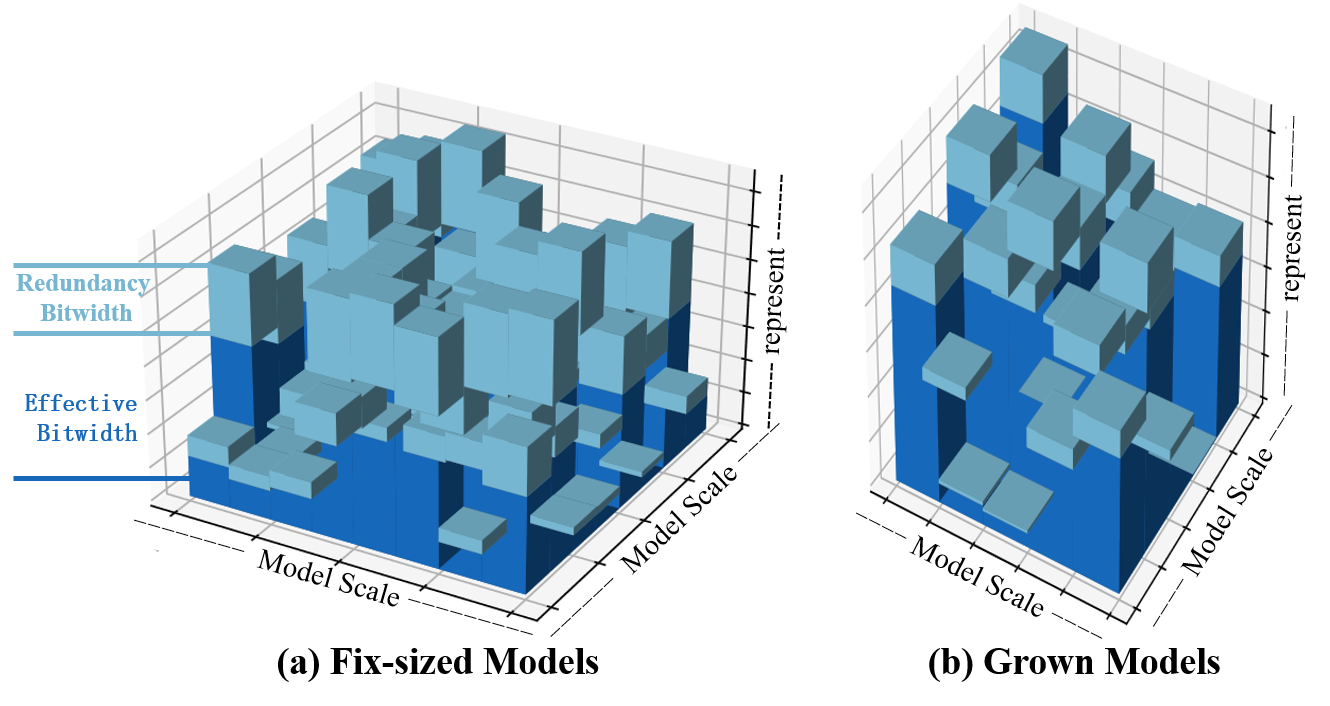
\includegraphics[width=0.8\textwidth]{imgs/bits.png}
\caption{Low Over-Parameterization in Grown Models}
\label{fig:low_overparam}
\end{figure}

In exploring growing models, this study has identified new challenges in quantization due to dynamic structural adjustments. growing models adapt their structures to meet specific task requirements, often resulting in relatively small model sizes. This reduction in model size diminishes over-parameterization \cite{over}, which typically facilitates successful quantization by accommodating the redundancy in parameters or bit-width. Over-parameterization allows for the removal of redundant parameters without significantly affecting model performance. However, because growing models are highly adapted to their tasks, they have fewer redundant parameters, making them more sensitive to quantization errors and prone to performance degradation. Figure \ref{fig:low_overparam} illustrates the phenomenon of low over-parameterization in growing models.

Additionally, convolutional neural networks that employ a structural re-parameterization strategy for width growing encounter further quantization difficulties. During re-parameterization, different-sized convolution kernels merge into the largest kernel size, such as combining 5×5, 3×3, and 1×1 kernels into a 5×5 kernel. This process leads to the center area of the merged kernel accumulating amplified parameter values, resulting in a highly non-uniform parameter distribution \cite{repopt}. This distribution diverges from the Gaussian or uniform distributions typically assumed by quantization strategies, forming a high-variance spike distribution. The central values of the convolution kernel become disproportionately important, increasing quantization sensitivity. Quantizing these high-magnitude values causes significant performance loss, as shown in Figure \ref{fig:sharp_weight_dist}.

\begin{figure}[ht]
\centering
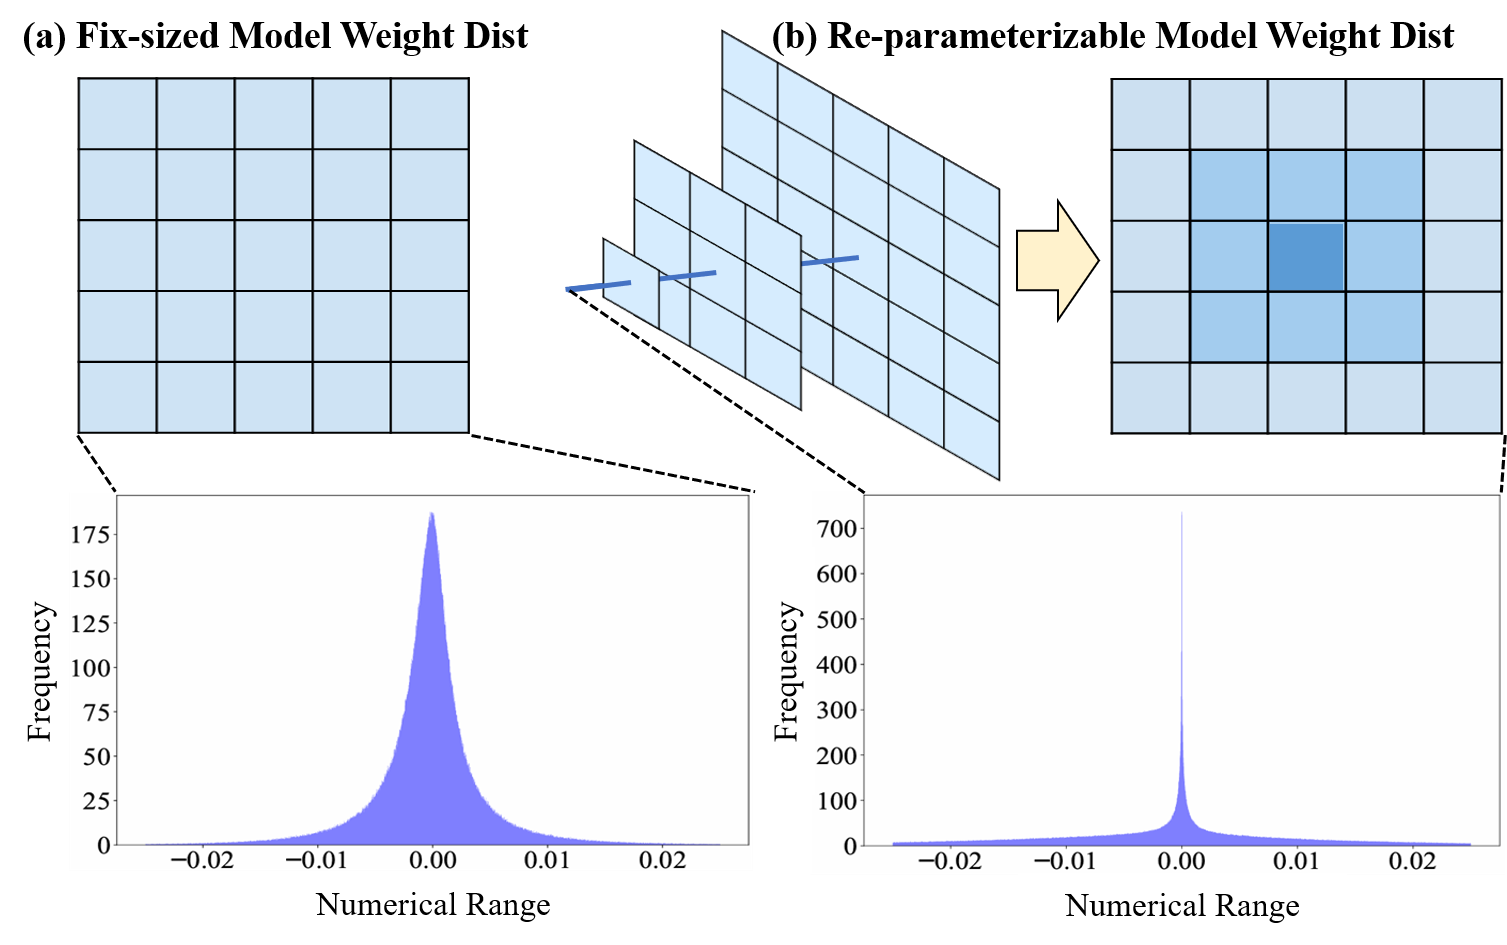
\includegraphics[width=0.8\textwidth]{imgs/rep.png}
\caption{Sharp Weight Distribution in Re-Parameterized Models}
\label{fig:sharp_weight_dist}
\end{figure}

In summary, the structural characteristics of growing models introduce additional challenges in the quantization process. The reduced model size decreases the room for over-parameterization, and the re-parameterization strategy creates a non-uniform weight distribution. Both factors adversely affect the efficiency and effectiveness of quantization. Therefore, to effectively quantize growing models, further exploration and development of specialized quantization strategies are necessary to address these unique challenges.

\subsection{Error Compensation}

To address the potential high quantization error in growing models, this study proposes an error compensation strategy aimed at mitigating overall quantization errors. The core of this strategy involves initially quantizing a portion of the model's parameters and calculating the resultant quantization errors. Subsequently, based on optimization principles, the unquantized parameters are selectively adjusted to compensate for these errors. This iterative optimization approach seeks to minimize the adverse effects of quantization, maintaining model performance while facilitating efficient quantization deployment in resource-constrained environments.

The primary error compensation method employed in this study is the Optimal Brain Surgeon (OBS) \cite{obs}, a second-order approximation technique based on the Hessian matrix, focused on minimizing performance loss due to parameter quantization. OBS determines the impact of parameter adjustments on model performance by analyzing the second derivatives of the loss function, allowing for targeted compression or adjustment of parameters to preserve overall model stability. For a convolutional or fully connected layer with \(X_l\) as input data and \(W_l\) as parameters, the optimization objective for the compressed weights \(\hat{W}_l\) is:

\begin{equation}
{\rm argmin}_{\hat{W}_l} \left\| W_lX_l - \hat{W}_lX_l \right\|_2^2
\end{equation}

Based on OBS theory, the quantization compression optimization results in the following conclusions:

\begin{equation}
w_p = {\rm argmin}_{w_p} \frac{\left(\mathrm{quant}(w_p) - w_p\right)^2}{\left[H^{-1}\right]_{pp}}
\end{equation}

\begin{equation}
\delta_p = -\frac{w_p - \mathrm{quant}(w_p)}{\left[H^{-1}\right]_{pp}} H_{:,p}^{-1}
\end{equation}


Here, \(w_p\) represents the weight to be quantized, and \(\mathrm{quant}(w_p)\) is the quantized weight value. \(\delta_p\) denotes the adjustment needed for the unquantized weights post-quantization, i.e., \(w_{p:} = w_{p:} - \delta_p\). \(H\) is the Hessian matrix, typically approximated by \(\mathbf{XX}^T\), where \(X\) can be a small subset of the training data used as a calibration set.

In the quantization process for growing models, this method effectively compensates for quantization-induced errors by purposefully adjusting the unquantized parameters, thereby reducing overall quantization errors and mitigating potential performance degradation. This approach ensures the efficient quantization of growing models, preserving their performance in resource-limited deployment scenarios.

\subsection{Weight Reordering}

While weight adjustments can partially mitigate the performance degradation caused by quantization errors in growing models, the conventional error compensation method does not account for the structural re-parameterization-based simulated width growing. This limitation makes it challenging to effectively apply error compensation to growing convolutional neural networks.

During structural re-parameterization, parameters at the central positions of the convolution kernels accumulate more computational contributions compared to those at the edges. This results in a weight distribution with heightened central importance. This phenomenon occurs because central parameters integrate information from multiple convolution paths, receiving inputs from various kernels, thus playing a more crucial role in the overall network representation. Conversely, edge parameters are linked to local input information, making them less significant. Consequently, the weight distribution deviates from the typical uniform or Gaussian distribution, forming a high-variance, sharp peak at the center.

In growing CNNs, central weights become even more critical, contributing significantly more to model performance. Standard quantization strategies that uniformly compress weights introduce substantial errors when applied indiscriminately across the entire weight matrix, leading to performance degradation.

To address this, we focus on the importance metric \(\frac{\left(\mathrm{quant}\left(w_p\right)-w_p\right)^2}{\left[H^{-1}\right]_{pp}}\). We propose a method to maintain the original sequential quantization logic while temporarily repositioning the most important central weights to the first column, quantizing them first. This approach allows more unquantized weights to adjust and compensate for the initial quantization errors. This logic extends to "sub-central" weights, where entire columns are repositioned and reordered based on importance metrics before quantization. This ensures that the most critical parameters are quantized first, with more unquantized parameters available to compensate for errors, enhancing the quantization process's effectiveness.

\begin{figure}[ht]
\centering
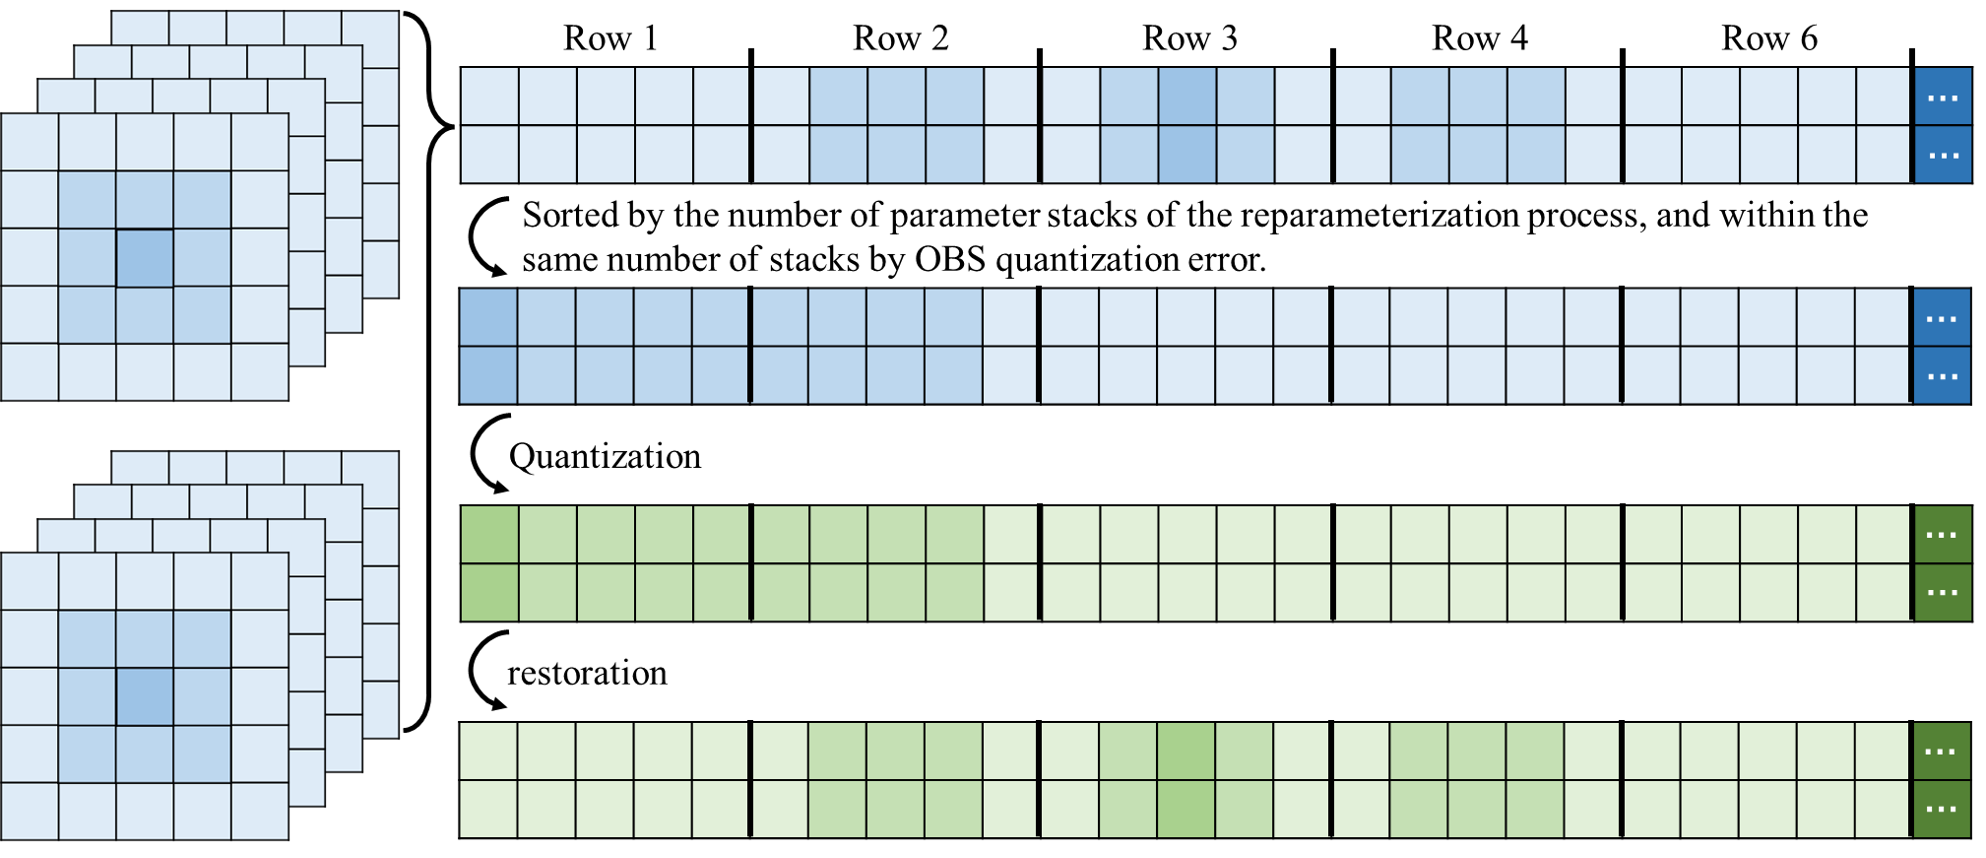
\includegraphics[width=\textwidth]{imgs/quant.png}
\caption{Quantization process of growing models based on error compensation and weight reordering}
\label{fig:quantization}
\end{figure}

Figure \ref{fig:quantization} illustrates this process for a convolution layer with parameter shape \([2, 4, 5, 5]\). Before quantization, the parameters are unfolded along the input channel dimension into a matrix of shape \([2, 100]\). The weights are then reordered based on their accumulation frequency during structural re-parameterization. Within each accumulation frequency, weights are internally reordered according to their importance metrics. This reordering creates a matrix ready for sequential quantization and error compensation. After quantization, the weights are reordered back to their original configuration and reshaped to \([2, 4, 5, 5]\).

By optimizing the quantization sequence based on error compensation and weight reordering, this approach significantly reduces quantization errors in growing CNNs, mitigating performance loss and providing an efficient solution for compressing and deploying growing models.


\subsection{Quantified Acceleration Practices for Grown Models}

An in-depth analysis of the quantization challenges faced by growing models and the proposed optimization strategies to address these challenges have been conducted. This section presents the practical quantization results of growing models on different hardware platforms, specifically the AMD EPYC 7642 128G 96-core CPU and the NVIDIA RTX 4090 24GB GPU. The selected growing network models is AdaGrow-Basic-ResNet, evaluated on the CIFAR-10 dataset. These models undergo three different quantization bit-width treatments: Floatpoint-16 (FP16), Integer-8 (INT8), and Weight-Integer-4-Activation-Floatpoint-16 (W4A16), with inference executed using Pytorch or TensorRT \cite{trt} backend. This demonstrates the application potential and efficiency of growing networks in real deployment environments.

\begin{table}[ht]
\centering
\tiny
\renewcommand{\arraystretch}{1.3}
\begin{adjustbox}{center}
\begin{tabular}{cccccccc}
\hline
\textbf{Model} & \textbf{Quantization} & \textbf{Bit-width} & \textbf{Backend} & \textbf{CPU Latency} & \textbf{GPU Latency} & \textbf{Acc\%} \\
 & \textbf{Method} & & & \textbf{(ms)} & \textbf{(ms)} & \\
\hline
ResNet-50 & Direct & FP32 & Pytorch & 10.95 & 3.52 & 86.12 \\
 & & FP32 & TensorRT & - & 948.63$\mu$s & 86.12 \\
 & & FP16 & TensorRT & - & 693.50$\mu$s & 86.48 \\
 & & INT8 & TensorRT & - & 675.65$\mu$s & 85.91 \\
 & & W4A16 & Pytorch & - & 3.05 & 85.04 \\
\hline
AdaGrow-Basic-ResNet & Direct & FP32 & Pytorch & 2.94 & 1.39 & 93.14 \\
 & & FP32 & TensorRT & - & 261.11$\mu$s & 93.14 \\
 & & FP16 & TensorRT & - & 166.46$\mu$s & 93.06 \\
 & & INT8 & TensorRT & - & 155.88$\mu$s & 92.27 \\
 & & W4A16 & Pytorch & - & 1.03 & 89.13 \\
\hline
AdaGrow-Basic-ResNet & OBS & FP32 & Pytorch & 2.94 & 1.39 & 93.14 \\
 & & FP32 & TensorRT & - & 261.11$\mu$s & 93.14 \\
 & & FP16 & TensorRT & - & 166.46$\mu$s & 93.12 \\
 & & INT8 & TensorRT & - & 155.88$\mu$s & 92.56 \\
 & & W4A16 & Pytorch & - & 1.03 & 91.66 \\
\hline
AdaGrow-Basic-ResNet & Proposed & FP32 & Pytorch & 2.94 & 1.39 & 93.14 \\
 & & FP32 & TensorRT & - & 261.11$\mu$s & 93.14 \\
 & & FP16 & TensorRT & - & 166.46$\mu$s & 93.16 \\
 & & INT8 & TensorRT & - & 155.88$\mu$s & 93.05 \\
 & & W4A16 & Pytorch & - & 1.03 & 92.98 \\
\hline
\end{tabular}
\end{adjustbox}
\caption{Quantization and Acceleration of growing CNNs}
\label{table:quantization}
\end{table}

Table \ref{table:quantization} presents the quantization and acceleration results of growing CNNs. The fixed-size baseline model, ResNet-50, shows robust quantization performance with minimal loss, demonstrating good quantization robustness. Conversely, the growing model AdaGrow-Basic-ResNet exhibits significant performance loss after direct quantization, aligning with the challenges discussed in Section \ref{challenge}. When directly quantized at FP16 and INT8 precision, AdaGrow-Basic-ResNet experiences performance degradation. However, the OBS method and the proposed error compensation and weight reordering strategy effectively reduce performance loss, with the latter showing superior results. At the stringent W4A16 precision, the proposed method significantly improves quantization accuracy, surpassing the OBS method, validating its effectiveness. Regarding inference latency, the growing model optimized with TensorRT exhibits a fourfold speedup over ResNet-50, indicating that the simplified model structure benefits subsequent compilation optimizations, showcasing the potential of growing models in inference acceleration.

\section{Limitation and Future Work}

While this study has achieved good dataset adaptability and an ideal performance-efficiency balance, there are still areas for improvement:

\textbf{Target Performance-Based Growing Termination Strategy}: The current growing model framework lacks a mechanism to stop growing based on a predefined performance target. Setting a specific performance goal and automatically deciding when to stop model growing would be highly convenient and practical for users. This requires designing a mechanism to predict the final performance of the current model structure once training converges. Future work will introduce an innovative solution by constructing and training an auxiliary predictive model to forecast the potential performance level of the network after training. The challenge lies in effectively collecting and utilizing data on the relationship between model structure and its final performance, ensuring that the predictive model can generalize across tasks.

\textbf{Enhanced Quantization with Dynamic Weight Reordering}: The current quantization method, based on error compensation and weight reordering, involves reordering weights by their structural re-parameterization accumulation counts and quantization error magnitude, followed by sequential weight quantization and adjustment of unquantized weights. After each error adjustment, the importance distribution of unquantized weight columns may change. Due to complexity considerations, this study did not further reorder weights based on the new importance metrics. Future work will continue to explore this area, aiming to dynamically adjust weight reordering during the quantization process to further minimize performance loss.

\section{Conclusions}

To address the need for optimizing neural network performance and inference efficiency under specific dataset conditions, this study proposes a growing model framework. By gradually expanding the model during training, it adaptively achieves the optimal architecture for a given dataset, resulting in higher recognition accuracy and faster inference speed. This framework offers a new solution for the efficient deployment of neural network models.

\textbf{AdaGrow Growing Training Paradigm}: The proposed growing training paradigm aims to achieve dataset-specific adaptability and an ideal performance-efficiency balance by gradually increasing the network's size. The study thoroughly explores key factors of network growing, including depth and width growing methods, growing frequency, growing termination conditions, single-growing scale, initialization methods for new modules, and optimizer adjustment strategies. Based on these explorations, an optimal growing model framework is constructed. Notably, the study employs structural re-parameterization techniques to simulate width growing in convolutional neural networks avoiding efficiency losses associated with direct width increases. The proposed framework achieves outstanding performance and efficiency on specific datasets and simplifies the regularization, learning rate adjustment, and optimizer design during training, significantly enhancing training efficiency and demonstrating broad practical value.

\textbf{Quantization Challenges and Solutions}: The study identifies challenges in quantizing growing models, such as the lack of over-parameterization and abnormal weight distributions caused by structural re-parameterization in CNNs, which can lead to significant quantization errors and affect post-quantization model performance. To address these challenges, the study proposes an innovative quantization method based on error compensation and weight reordering. This method effectively reduces performance losses due to quantization, providing a new solution for efficiently quantizing growing models.

Extensive experimental validation demonstrates that the proposed growing model framework excels in various tasks across computer vision datasets, showcasing its superior performance and efficiency. Additionally, the proposed quantization method, based on error compensation and weight reordering, successfully applies to many CNN models, enabling more efficient quantization compression with minimal performance loss. These achievements offer a new technical pathway for efficient training and inference of dataset-adaptive models.

\bibliographystyle{elsarticle-num} 
\bibliography{ref}

\end{document}
